\documentclass[11pt,a4paper]{article}

\usepackage{fullpage}
\usepackage{hyperref}
\usepackage{graphicx}
\usepackage{subcaption}
\usepackage{float}
\usepackage{amsmath}
\usepackage{bm}
\usepackage{booktabs}

\usepackage{amsmath}
\usepackage{tikz}
\usepackage{mathdots}
\usepackage{cancel}
\usepackage{color}
\usepackage{siunitx}
\usepackage{array}
\usepackage{multirow}
\usepackage{amssymb}
\usepackage{gensymb}
\usetikzlibrary{fadings}
\usetikzlibrary{patterns}

%\pdfcompresslevel=2
%\pdfobjcompresslevel=2




\usepackage{fancyhdr}
\pagestyle{fancy}
\fancyhf{}
\usepackage{todonotes}                %% notes from the authors

\renewcommand{\headrulewidth}{0pt}
\renewcommand{\footrulewidth}{0pt}

\fancypagestyle{firstpagefooter} {
	\lfoot{\tiny{Version: 25.09.2018}}
	\cfoot{}
	\rfoot{\thepage}
	
}


\renewcommand{\t}[1]{%
	{\texttt{#1}}}



\lfoot{Name: Luca\_Di\_Bartolomeo Legi: 18-961-053}
\rfoot{\thepage}

\begin{document}

\setlength{\pdfpxdimen}{1in/150} % Define resolution of PDF
\title{Advanced Systems Lab Report\\ \normalsize{Autumn Semester 2018}}
\author{Name: Luca\_Di\_Bartolomeo\\Legi: 18-961-053}
\date{
	\vspace{4cm}
	\textbf{Grading} \\
	\vspace{0.5cm}
	\begin{tabular}{|c|c|}
		\hline  \textbf{Section} & \textbf{Points} \\
		\hline  1                &                 \\ 
		\hline  2                &                 \\ 
		\hline  3                &                 \\ 
		\hline  4                &                 \\ 
		\hline  5                &                 \\ 
		\hline  6                &                 \\ 
		\hline  7                &                 \\ 
		\hline \hline Total      &                 \\
		\hline 
	\end{tabular} 
}
\maketitle
\thispagestyle{firstpagefooter}

\newpage

\section{System Overview (75 pts)}

This section will explain the general functionality of the middleware. It will also explain
how requests are parsed and forwarded to the servers.

\subsection{System architecture}

\tikzset{every picture/.style={line width=0.75pt}} %set default line width to 0.75pt
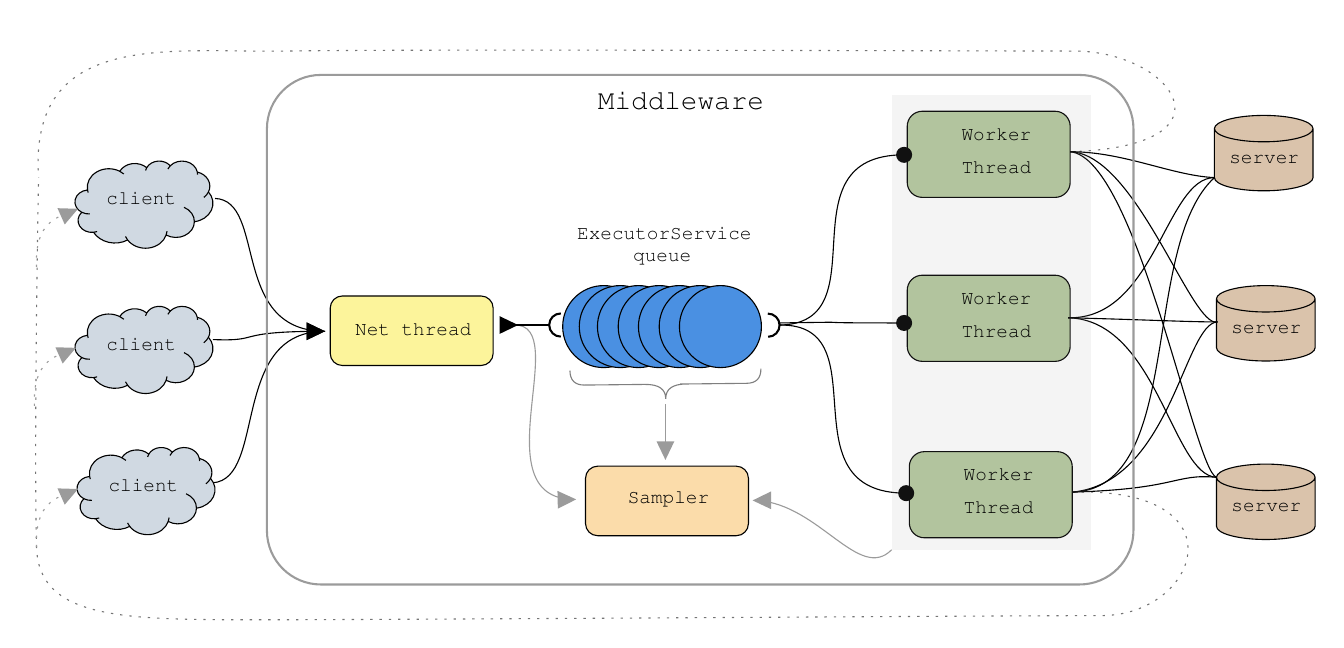
\begin{tikzpicture}[x=0.75pt,y=0.75pt,yscale=-1,xscale=1]
%uncomment if require: \path (0,333); %set diagram left start at 0, and has height of 333
%Curve Lines [id:da8207420048585989]
\draw [color={rgb, 255:red, 155; green, 155; blue, 155 }  ,draw opacity=1 ]   (246.5,145) .. controls (275.21,144.01) and (230.41,228.29) .. (275.12,229) ;
\draw [shift={(276.5,229)}, rotate = 538.78] [fill={rgb, 255:red, 155; green, 155; blue, 155 }  ,fill opacity=1 ][line width=0.75]  [draw opacity=0] (8.93,-4.29) -- (0,0) -- (8.93,4.29) -- cycle    ;
%Flowchart: Magnetic Disk [id:dp31865808226302494]
\draw  [fill={rgb, 255:red, 218; green, 195; blue, 171 }  ,fill opacity=1 ] (631.5,50.36) -- (631.5,73.97) .. controls (631.5,77.49) and (620.87,80.33) .. (607.75,80.33) .. controls (594.63,80.33) and (584,77.49) .. (584,73.97) -- (584,50.36)(631.5,50.36) .. controls (631.5,53.87) and (620.87,56.72) .. (607.75,56.72) .. controls (594.63,56.72) and (584,53.87) .. (584,50.36) .. controls (584,46.85) and (594.63,44) .. (607.75,44) .. controls (620.87,44) and (631.5,46.85) .. (631.5,50.36) -- cycle ;
%Flowchart: Magnetic Disk [id:dp18742640338889216]
\draw  [fill={rgb, 255:red, 218; green, 195; blue, 171 }  ,fill opacity=1 ] (632.5,132.36) -- (632.5,155.97) .. controls (632.5,159.49) and (621.87,162.33) .. (608.75,162.33) .. controls (595.63,162.33) and (585,159.49) .. (585,155.97) -- (585,132.36)(632.5,132.36) .. controls (632.5,135.87) and (621.87,138.72) .. (608.75,138.72) .. controls (595.63,138.72) and (585,135.87) .. (585,132.36) .. controls (585,128.85) and (595.63,126) .. (608.75,126) .. controls (621.87,126) and (632.5,128.85) .. (632.5,132.36) -- cycle ;
%Flowchart: Magnetic Disk [id:dp004533420186562553]
\draw  [fill={rgb, 255:red, 218; green, 195; blue, 171 }  ,fill opacity=1 ] (632.5,218.36) -- (632.5,241.97) .. controls (632.5,245.49) and (621.87,248.33) .. (608.75,248.33) .. controls (595.63,248.33) and (585,245.49) .. (585,241.97) -- (585,218.36)(632.5,218.36) .. controls (632.5,221.87) and (621.87,224.72) .. (608.75,224.72) .. controls (595.63,224.72) and (585,221.87) .. (585,218.36) .. controls (585,214.85) and (595.63,212) .. (608.75,212) .. controls (621.87,212) and (632.5,214.85) .. (632.5,218.36) -- cycle ;
%Shape: Cloud [id:dp4220513027642627]
\draw  [fill={rgb, 255:red, 75; green, 109; blue, 142 }  ,fill opacity=0.26 ] (41.05,79.83) .. controls (40.52,76.44) and (42.27,73.09) .. (45.58,71.19) .. controls (48.89,69.3) and (53.16,69.19) .. (56.59,70.92) .. controls (57.8,68.95) and (60.02,67.59) .. (62.58,67.25) .. controls (65.14,66.91) and (67.73,67.63) .. (69.58,69.2) .. controls (70.61,67.41) and (72.64,66.21) .. (74.95,66.03) .. controls (77.26,65.84) and (79.51,66.69) .. (80.92,68.27) .. controls (82.79,66.38) and (85.76,65.58) .. (88.55,66.23) .. controls (91.34,66.87) and (93.45,68.84) .. (93.96,71.28) .. controls (96.25,71.82) and (98.16,73.19) .. (99.19,75.03) .. controls (100.22,76.87) and (100.28,79.01) .. (99.34,80.89) .. controls (101.6,83.41) and (102.13,86.78) .. (100.73,89.73) .. controls (99.33,92.67) and (96.22,94.76) .. (92.56,95.22) .. controls (92.53,97.98) and (90.77,100.52) .. (87.95,101.85) .. controls (85.13,103.19) and (81.69,103.11) .. (78.96,101.64) .. controls (77.79,104.95) and (74.52,107.39) .. (70.55,107.9) .. controls (66.58,108.41) and (62.62,106.9) .. (60.39,104.02) .. controls (57.66,105.44) and (54.38,105.85) .. (51.29,105.16) .. controls (48.2,104.46) and (45.57,102.72) .. (43.98,100.33) .. controls (41.19,100.61) and (38.48,99.37) .. (37.22,97.21) .. controls (35.95,95.06) and (36.38,92.45) .. (38.3,90.69) .. controls (35.81,89.43) and (34.54,86.92) .. (35.15,84.48) .. controls (35.76,82.04) and (38.12,80.22) .. (40.99,79.96) ; \draw   (38.31,90.69) .. controls (39.48,91.29) and (40.84,91.56) .. (42.2,91.47)(43.98,100.33) .. controls (44.56,100.28) and (45.14,100.15) .. (45.68,99.96)(60.39,104.02) .. controls (59.98,103.49) and (59.64,102.92) .. (59.36,102.33)(78.96,101.64) .. controls (79.17,101.04) and (79.31,100.41) .. (79.37,99.78)(92.56,95.22) .. controls (92.59,92.27) and (90.64,89.57) .. (87.56,88.28)(99.34,80.89) .. controls (98.84,81.89) and (98.08,82.78) .. (97.12,83.49)(93.96,71.28) .. controls (94.05,71.69) and (94.09,72.1) .. (94.08,72.51)(80.92,68.27) .. controls (80.45,68.75) and (80.07,69.27) .. (79.78,69.84)(69.58,69.2) .. controls (69.33,69.63) and (69.14,70.08) .. (69.03,70.55)(56.59,70.92) .. controls (57.31,71.28) and (57.98,71.72) .. (58.58,72.23)(41.05,79.83) .. controls (41.13,80.29) and (41.24,80.76) .. (41.4,81.21) ;
%Shape: Cloud [id:dp5696976331398176]
\draw  [fill={rgb, 255:red, 75; green, 109; blue, 142 }  ,fill opacity=0.26 ] (41.05,149.83) .. controls (40.52,146.44) and (42.27,143.09) .. (45.58,141.19) .. controls (48.89,139.3) and (53.16,139.19) .. (56.59,140.92) .. controls (57.8,138.95) and (60.02,137.59) .. (62.58,137.25) .. controls (65.14,136.91) and (67.73,137.63) .. (69.58,139.2) .. controls (70.61,137.41) and (72.64,136.21) .. (74.95,136.03) .. controls (77.26,135.84) and (79.51,136.69) .. (80.92,138.27) .. controls (82.79,136.38) and (85.76,135.58) .. (88.55,136.23) .. controls (91.34,136.87) and (93.45,138.84) .. (93.96,141.28) .. controls (96.25,141.82) and (98.16,143.19) .. (99.19,145.03) .. controls (100.22,146.87) and (100.28,149.01) .. (99.34,150.89) .. controls (101.6,153.41) and (102.13,156.78) .. (100.73,159.73) .. controls (99.33,162.67) and (96.22,164.76) .. (92.56,165.22) .. controls (92.53,167.98) and (90.77,170.52) .. (87.95,171.85) .. controls (85.13,173.19) and (81.69,173.11) .. (78.96,171.64) .. controls (77.79,174.95) and (74.52,177.39) .. (70.55,177.9) .. controls (66.58,178.41) and (62.62,176.9) .. (60.39,174.02) .. controls (57.66,175.44) and (54.38,175.85) .. (51.29,175.16) .. controls (48.2,174.46) and (45.57,172.72) .. (43.98,170.33) .. controls (41.19,170.61) and (38.48,169.37) .. (37.22,167.21) .. controls (35.95,165.06) and (36.38,162.45) .. (38.3,160.69) .. controls (35.81,159.43) and (34.54,156.92) .. (35.15,154.48) .. controls (35.76,152.04) and (38.12,150.22) .. (40.99,149.96) ; \draw   (38.31,160.69) .. controls (39.48,161.29) and (40.84,161.56) .. (42.2,161.47)(43.98,170.33) .. controls (44.56,170.28) and (45.14,170.15) .. (45.68,169.96)(60.39,174.02) .. controls (59.98,173.49) and (59.64,172.92) .. (59.36,172.33)(78.96,171.64) .. controls (79.17,171.04) and (79.31,170.41) .. (79.37,169.78)(92.56,165.22) .. controls (92.59,162.27) and (90.64,159.57) .. (87.56,158.28)(99.34,150.89) .. controls (98.84,151.89) and (98.08,152.78) .. (97.12,153.49)(93.96,141.28) .. controls (94.05,141.69) and (94.09,142.1) .. (94.08,142.51)(80.92,138.27) .. controls (80.45,138.75) and (80.07,139.27) .. (79.78,139.84)(69.58,139.2) .. controls (69.33,139.63) and (69.14,140.08) .. (69.03,140.55)(56.59,140.92) .. controls (57.31,141.28) and (57.98,141.72) .. (58.58,142.23)(41.05,149.83) .. controls (41.13,150.29) and (41.24,150.76) .. (41.4,151.21) ;
%Shape: Cloud [id:dp4190382420411689]
\draw  [fill={rgb, 255:red, 75; green, 109; blue, 142 }  ,fill opacity=0.26 ] (42.05,217.83) .. controls (41.52,214.44) and (43.27,211.09) .. (46.58,209.19) .. controls (49.89,207.3) and (54.16,207.19) .. (57.59,208.92) .. controls (58.8,206.95) and (61.02,205.59) .. (63.58,205.25) .. controls (66.14,204.91) and (68.73,205.63) .. (70.58,207.2) .. controls (71.61,205.41) and (73.64,204.21) .. (75.95,204.03) .. controls (78.26,203.84) and (80.51,204.69) .. (81.92,206.27) .. controls (83.79,204.38) and (86.76,203.58) .. (89.55,204.23) .. controls (92.34,204.87) and (94.45,206.84) .. (94.96,209.28) .. controls (97.25,209.82) and (99.16,211.19) .. (100.19,213.03) .. controls (101.22,214.87) and (101.28,217.01) .. (100.34,218.89) .. controls (102.6,221.41) and (103.13,224.78) .. (101.73,227.73) .. controls (100.33,230.67) and (97.22,232.76) .. (93.56,233.22) .. controls (93.53,235.98) and (91.77,238.52) .. (88.95,239.85) .. controls (86.13,241.19) and (82.69,241.11) .. (79.96,239.64) .. controls (78.79,242.95) and (75.52,245.39) .. (71.55,245.9) .. controls (67.58,246.41) and (63.62,244.9) .. (61.39,242.02) .. controls (58.66,243.44) and (55.38,243.85) .. (52.29,243.16) .. controls (49.2,242.46) and (46.57,240.72) .. (44.98,238.33) .. controls (42.19,238.61) and (39.48,237.37) .. (38.22,235.21) .. controls (36.95,233.06) and (37.38,230.45) .. (39.3,228.69) .. controls (36.81,227.43) and (35.54,224.92) .. (36.15,222.48) .. controls (36.76,220.04) and (39.12,218.22) .. (41.99,217.96) ; \draw   (39.31,228.69) .. controls (40.48,229.29) and (41.84,229.56) .. (43.2,229.47)(44.98,238.33) .. controls (45.56,238.28) and (46.14,238.15) .. (46.68,237.96)(61.39,242.02) .. controls (60.98,241.49) and (60.64,240.92) .. (60.36,240.33)(79.96,239.64) .. controls (80.17,239.04) and (80.31,238.41) .. (80.37,237.78)(93.56,233.22) .. controls (93.59,230.27) and (91.64,227.57) .. (88.56,226.28)(100.34,218.89) .. controls (99.84,219.89) and (99.08,220.78) .. (98.12,221.49)(94.96,209.28) .. controls (95.05,209.69) and (95.09,210.1) .. (95.08,210.51)(81.92,206.27) .. controls (81.45,206.75) and (81.07,207.27) .. (80.78,207.84)(70.58,207.2) .. controls (70.33,207.63) and (70.14,208.08) .. (70.03,208.55)(57.59,208.92) .. controls (58.31,209.28) and (58.98,209.72) .. (59.58,210.23)(42.05,217.83) .. controls (42.13,218.29) and (42.24,218.76) .. (42.4,219.21) ;
%Flowchart: Alternative Process [id:dp3695411950817773]
\draw  [fill={rgb, 255:red, 248; green, 231; blue, 28 }  ,fill opacity=0.44 ] (158,136.86) .. controls (158,133.62) and (160.62,131) .. (163.86,131) -- (230.64,131) .. controls (233.88,131) and (236.5,133.62) .. (236.5,136.86) -- (236.5,158.64) .. controls (236.5,161.88) and (233.88,164.5) .. (230.64,164.5) -- (163.86,164.5) .. controls (160.62,164.5) and (158,161.88) .. (158,158.64) -- cycle ;
%Flowchart: Alternative Process [id:dp8619535575878048]
\draw  [fill={rgb, 255:red, 65; green, 117; blue, 5 }  ,fill opacity=0.39 ] (436,49.26) .. controls (436,45.25) and (439.25,42) .. (443.26,42) -- (507.24,42) .. controls (511.25,42) and (514.5,45.25) .. (514.5,49.26) -- (514.5,76.24) .. controls (514.5,80.25) and (511.25,83.5) .. (507.24,83.5) -- (443.26,83.5) .. controls (439.25,83.5) and (436,80.25) .. (436,76.24) -- cycle ;
%Flowchart: Alternative Process [id:dp22606581491296263]
\draw  [fill={rgb, 255:red, 65; green, 117; blue, 5 }  ,fill opacity=0.39 ] (436,128.26) .. controls (436,124.25) and (439.25,121) .. (443.26,121) -- (507.24,121) .. controls (511.25,121) and (514.5,124.25) .. (514.5,128.26) -- (514.5,155.24) .. controls (514.5,159.25) and (511.25,162.5) .. (507.24,162.5) -- (443.26,162.5) .. controls (439.25,162.5) and (436,159.25) .. (436,155.24) -- cycle ;
%Flowchart: Alternative Process [id:dp8763167525219511]
\draw  [fill={rgb, 255:red, 65; green, 117; blue, 5 }  ,fill opacity=0.39 ] (437,213.26) .. controls (437,209.25) and (440.25,206) .. (444.26,206) -- (508.24,206) .. controls (512.25,206) and (515.5,209.25) .. (515.5,213.26) -- (515.5,240.24) .. controls (515.5,244.25) and (512.25,247.5) .. (508.24,247.5) -- (444.26,247.5) .. controls (440.25,247.5) and (437,244.25) .. (437,240.24) -- cycle ;
%Shape: Circle [id:dp5254909806920878]
\draw  [fill={rgb, 255:red, 74; green, 144; blue, 226 }  ,fill opacity=1 ] (270,145.75) .. controls (270,134.84) and (278.84,126) .. (289.75,126) .. controls (300.66,126) and (309.5,134.84) .. (309.5,145.75) .. controls (309.5,156.66) and (300.66,165.5) .. (289.75,165.5) .. controls (278.84,165.5) and (270,156.66) .. (270,145.75) -- cycle ;
%Shape: Circle [id:dp7403438704054486]
\draw  [fill={rgb, 255:red, 74; green, 144; blue, 226 }  ,fill opacity=1 ] (278,145.75) .. controls (278,134.84) and (286.84,126) .. (297.75,126) .. controls (308.66,126) and (317.5,134.84) .. (317.5,145.75) .. controls (317.5,156.66) and (308.66,165.5) .. (297.75,165.5) .. controls (286.84,165.5) and (278,156.66) .. (278,145.75) -- cycle ;
%Shape: Circle [id:dp5947829779233558]
\draw  [fill={rgb, 255:red, 74; green, 144; blue, 226 }  ,fill opacity=1 ] (286.75,145.75) .. controls (286.75,134.84) and (295.59,126) .. (306.5,126) .. controls (317.41,126) and (326.25,134.84) .. (326.25,145.75) .. controls (326.25,156.66) and (317.41,165.5) .. (306.5,165.5) .. controls (295.59,165.5) and (286.75,156.66) .. (286.75,145.75) -- cycle ;
%Shape: Circle [id:dp38875641792120796]
\draw  [fill={rgb, 255:red, 74; green, 144; blue, 226 }  ,fill opacity=1 ] (296.75,145.75) .. controls (296.75,134.84) and (305.59,126) .. (316.5,126) .. controls (327.41,126) and (336.25,134.84) .. (336.25,145.75) .. controls (336.25,156.66) and (327.41,165.5) .. (316.5,165.5) .. controls (305.59,165.5) and (296.75,156.66) .. (296.75,145.75) -- cycle ;
%Shape: Circle [id:dp9984262829491981]
\draw  [fill={rgb, 255:red, 74; green, 144; blue, 226 }  ,fill opacity=1 ] (306.5,145.75) .. controls (306.5,134.84) and (315.34,126) .. (326.25,126) .. controls (337.16,126) and (346,134.84) .. (346,145.75) .. controls (346,156.66) and (337.16,165.5) .. (326.25,165.5) .. controls (315.34,165.5) and (306.5,156.66) .. (306.5,145.75) -- cycle ;
%Shape: Circle [id:dp5714364782996804]
\draw  [fill={rgb, 255:red, 74; green, 144; blue, 226 }  ,fill opacity=1 ] (316.5,145.75) .. controls (316.5,134.84) and (325.34,126) .. (336.25,126) .. controls (347.16,126) and (356,134.84) .. (356,145.75) .. controls (356,156.66) and (347.16,165.5) .. (336.25,165.5) .. controls (325.34,165.5) and (316.5,156.66) .. (316.5,145.75) -- cycle ;
%Shape: Circle [id:dp20737960203860872]
\draw  [fill={rgb, 255:red, 74; green, 144; blue, 226 }  ,fill opacity=1 ] (326.25,145.75) .. controls (326.25,134.84) and (335.09,126) .. (346,126) .. controls (356.91,126) and (365.75,134.84) .. (365.75,145.75) .. controls (365.75,156.66) and (356.91,165.5) .. (346,165.5) .. controls (335.09,165.5) and (326.25,156.66) .. (326.25,145.75) -- cycle ;
%Flowchart: Alternative Process [id:dp09372660315036052]
\draw  [fill={rgb, 255:red, 245; green, 166; blue, 35 }  ,fill opacity=0.39 ] (281,218.86) .. controls (281,215.62) and (283.62,213) .. (286.86,213) -- (353.64,213) .. controls (356.88,213) and (359.5,215.62) .. (359.5,218.86) -- (359.5,240.64) .. controls (359.5,243.88) and (356.88,246.5) .. (353.64,246.5) -- (286.86,246.5) .. controls (283.62,246.5) and (281,243.88) .. (281,240.64) -- cycle ;
%Straight Lines [id:da004086798255003687]
\draw [color={rgb, 255:red, 155; green, 155; blue, 155 }  ,draw opacity=1 ]   (319.5,208) -- (319.5,183) ;
\draw [shift={(319.5,210)}, rotate = 270] [fill={rgb, 255:red, 155; green, 155; blue, 155 }  ,fill opacity=1 ][line width=0.75]  [draw opacity=0] (8.93,-4.29) -- (0,0) -- (8.93,4.29) -- cycle    ;
%Shape: Brace [id:dp6467285774957658]
\draw  [color={rgb, 255:red, 0; green, 0; blue, 0 }  ,draw opacity=0.5 ] (273.5,167) .. controls (273.55,171.67) and (275.91,173.97) .. (280.58,173.92) -- (309.58,173.61) .. controls (316.25,173.54) and (319.6,175.83) .. (319.65,180.5) .. controls (319.6,175.83) and (322.91,173.46) .. (329.58,173.39)(326.58,173.43) -- (358.58,173.08) .. controls (363.25,173.03) and (365.55,170.67) .. (365.5,166) ;
%Curve Lines [id:da34856425304843697]
\draw    (515.5,225.5) .. controls (570,224) and (548,106.97) .. (584,73.97) ;
%Curve Lines [id:da220505840939633]
\draw    (515.5,225.5) .. controls (563,221) and (569.5,144) .. (585.5,143.5) ;
%Curve Lines [id:da8572940071408939]
\draw    (515.5,225.5) .. controls (567,224) and (564.5,216.5) .. (585,218.36) ;
%Curve Lines [id:da633725450513456]
\draw    (513.5,141.5) .. controls (555.5,142.5) and (560.5,74) .. (584,73.97) ;
%Curve Lines [id:da7953196170830459]
\draw    (513.5,141.5) .. controls (556.5,142.5) and (563.5,217.5) .. (585,218.36) ;
%Curve Lines [id:da06591746606590854]
\draw    (513.5,141.5) .. controls (553.5,142.5) and (570.5,143.5) .. (585.5,143.5) ;
%Curve Lines [id:da4980062883183556]
\draw    (584,73.97) .. controls (563.5,73) and (540.5,61.5) .. (514.5,61.5) ;
%Curve Lines [id:da6636144272005104]
\draw    (514.5,61.5) .. controls (546.5,62.5) and (573,147.03) .. (585.5,143.5) ;
%Curve Lines [id:da06541793865828716]
\draw    (514.5,61.5) .. controls (546.5,64.5) and (574.5,215.5) .. (585,218.36) ;
%Curve Lines [id:da6020612171716928]
\draw [color={rgb, 255:red, 0; green, 0; blue, 0 }  ,draw opacity=0.54 ] [dash pattern={on 0.84pt off 2.51pt}]  (514.5,61.5) .. controls (597.5,59) and (563.5,13) .. (516.5,13) .. controls (469.5,13) and (195.5,12) .. (138.5,13) .. controls (81.5,14) and (12.5,2) .. (17.5,74) ;
%Curve Lines [id:da13425580569311601]
\draw [color={rgb, 255:red, 0; green, 0; blue, 0 }  ,draw opacity=0.54 ] [dash pattern={on 0.84pt off 2.51pt}]  (515.5,225.5) .. controls (598.5,223) and (576.5,285) .. (529.5,285) .. controls (482.5,285) and (190.5,287) .. (124.5,287) .. controls (58.5,287) and (17.5,287) .. (16.5,252) .. controls (15.5,217) and (16.5,121) .. (17.5,74) ;
%Curve Lines [id:da851077752428268]
\draw [color={rgb, 255:red, 155; green, 155; blue, 155 }  ,draw opacity=1 ] [dash pattern={on 0.84pt off 2.51pt}]  (16.5,252) .. controls (15.57,230.49) and (25.99,228.22) .. (34.71,224.75) ;
\draw [shift={(36.5,224)}, rotate = 516.04] [fill={rgb, 255:red, 155; green, 155; blue, 155 }  ,fill opacity=1 ][line width=0.75]  [draw opacity=0] (8.93,-4.29) -- (0,0) -- (8.93,4.29) -- cycle    ;
%Curve Lines [id:da9684791861681259]
\draw [color={rgb, 255:red, 155; green, 155; blue, 155 }  ,draw opacity=1 ] [dash pattern={on 0.84pt off 2.51pt}]  (15.5,184) .. controls (14.57,162.49) and (24.99,160.22) .. (33.71,156.75) ;
\draw [shift={(35.5,156)}, rotate = 516.04] [fill={rgb, 255:red, 155; green, 155; blue, 155 }  ,fill opacity=1 ][line width=0.75]  [draw opacity=0] (8.93,-4.29) -- (0,0) -- (8.93,4.29) -- cycle    ;
%Curve Lines [id:da5437042231934821]
\draw [color={rgb, 255:red, 155; green, 155; blue, 155 }  ,draw opacity=1 ] [dash pattern={on 0.84pt off 2.51pt}]  (16.5,117) .. controls (15.57,95.49) and (25.99,93.22) .. (34.71,89.75) ;
\draw [shift={(36.5,89)}, rotate = 516.04] [fill={rgb, 255:red, 155; green, 155; blue, 155 }  ,fill opacity=1 ][line width=0.75]  [draw opacity=0] (8.93,-4.29) -- (0,0) -- (8.93,4.29) -- cycle    ;
%Curve Lines [id:da7658814795004276]
\draw    (102.5,84) .. controls (127.25,84.99) and (109.86,146.75) .. (154.14,147.98) ;
\draw [shift={(155.5,148)}, rotate = 180] [fill={rgb, 255:red, 0; green, 0; blue, 0 }  ][line width=0.75]  [draw opacity=0] (8.93,-4.29) -- (0,0) -- (8.93,4.29) -- cycle    ;
%Curve Lines [id:da35021167492441974]
\draw    (101.5,152) .. controls (126.5,153) and (109.5,148) .. (155.5,148) ;
%Curve Lines [id:da296371158956537]
\draw    (101.5,221) .. controls (127.24,219.02) and (109.86,149.41) .. (154.14,148.02) ;
\draw [shift={(155.5,148)}, rotate = 180] [fill={rgb, 255:red, 0; green, 0; blue, 0 }  ][line width=0.75]  [draw opacity=0] (8.93,-4.29) -- (0,0) -- (8.93,4.29) -- cycle    ;
%Curve Lines [id:da6120043212049284]
\draw    (374.5,145) .. controls (424.25,144.25) and (374.5,63) .. (434.5,63) ;
\draw [shift={(434.5,63)}, rotate = 0] [color={rgb, 255:red, 0; green, 0; blue, 0 }  ][fill={rgb, 255:red, 0; green, 0; blue, 0 }  ][line width=0.75]      (0, 0) circle [x radius= 3.35, y radius= 3.35]   ;
\draw [shift={(374.5,145)}, rotate = 539.14] [color={rgb, 255:red, 0; green, 0; blue, 0 }  ][line width=0.75]      (5.59,-5.59) .. controls (2.5,-5.59) and (0,-3.09) .. (0,0) .. controls (0,3.09) and (2.5,5.59) .. (5.59,5.59) ;
%Shape: Rectangle [id:dp6393869074642782]
\draw  [color={rgb, 255:red, 155; green, 155; blue, 155 }  ,draw opacity=1 ][line width=0.75]  (127.5,50.5) .. controls (127.5,36.14) and (139.14,24.5) .. (153.5,24.5) -- (519,24.5) .. controls (533.36,24.5) and (545,36.14) .. (545,50.5) -- (545,244) .. controls (545,258.36) and (533.36,270) .. (519,270) -- (153.5,270) .. controls (139.14,270) and (127.5,258.36) .. (127.5,244) -- cycle ;
%Curve Lines [id:da5811038095898187]
\draw    (374.5,144) .. controls (424.25,143.25) and (374.5,144) .. (434.5,144) ;
\draw [shift={(434.5,144)}, rotate = 0] [color={rgb, 255:red, 0; green, 0; blue, 0 }  ][fill={rgb, 255:red, 0; green, 0; blue, 0 }  ][line width=0.75]      (0, 0) circle [x radius= 3.35, y radius= 3.35]   ;
%Curve Lines [id:da24462951940228672]
\draw    (374.5,145) .. controls (424.25,144.25) and (375.5,226) .. (435.5,226) ;
\draw [shift={(435.5,226)}, rotate = 0] [color={rgb, 255:red, 0; green, 0; blue, 0 }  ][fill={rgb, 255:red, 0; green, 0; blue, 0 }  ][line width=0.75]      (0, 0) circle [x radius= 3.35, y radius= 3.35]   ;
%Straight Lines [id:da14248278706791395]
\draw    (247.5,145) -- (263.5,145) ;
\draw [shift={(263.5,145)}, rotate = 0] [color={rgb, 255:red, 0; green, 0; blue, 0 }  ][line width=0.75]      (5.59,-5.59) .. controls (2.5,-5.59) and (0,-3.09) .. (0,0) .. controls (0,3.09) and (2.5,5.59) .. (5.59,5.59) ;
\draw [shift={(248.5,145)}, rotate = 180] [fill={rgb, 255:red, 0; green, 0; blue, 0 }  ][line width=0.75]  [draw opacity=0] (8.93,-4.29) -- (0,0) -- (8.93,4.29) -- cycle    ;
%Shape: Rectangle [id:dp5518128549851555]
\draw  [color={rgb, 255:red, 255; green, 255; blue, 255 }  ,draw opacity=0 ][fill={rgb, 255:red, 155; green, 155; blue, 155 }  ,fill opacity=0.11 ] (428.5,34) -- (524.5,34) -- (524.5,253.26) -- (428.5,253.26) -- cycle ;
%Curve Lines [id:da5224472977531855]
\draw [color={rgb, 255:red, 155; green, 155; blue, 155 }  ,draw opacity=1 ]   (363.8,229.56) .. controls (393.5,231.31) and (412.9,269.09) .. (428.5,253.26) ;
\draw [shift={(361.5,229.5)}, rotate = 359.69] [fill={rgb, 255:red, 155; green, 155; blue, 155 }  ,fill opacity=1 ][line width=0.75]  [draw opacity=0] (8.93,-4.29) -- (0,0) -- (8.93,4.29) -- cycle    ;
% Text Node
\draw (608,65) node  [align=left] {{\fontfamily{pcr}\selectfont {\scriptsize server}}};
% Text Node
\draw (609,147) node  [align=left] {{\fontfamily{pcr}\selectfont {\scriptsize server}}};
% Text Node
\draw (609,233) node  [align=left] {{\fontfamily{pcr}\selectfont {\scriptsize server}}};
% Text Node
\draw (67,84) node  [align=left] {{\fontfamily{pcr}\selectfont {\scriptsize client}}};
% Text Node
\draw (67,154) node  [align=left] {{\fontfamily{pcr}\selectfont {\scriptsize client}}};
% Text Node
\draw (68,222) node  [align=left] {{\fontfamily{pcr}\selectfont {\scriptsize client}}};
% Text Node
\draw (198,147) node  [align=left] {{\scriptsize {\fontfamily{pcr}\selectfont Net thread}}};
% Text Node
\draw (479,61) node  [align=left] {{\scriptsize {\fontfamily{pcr}\selectfont Worker }}\\{\scriptsize {\fontfamily{pcr}\selectfont Thread}}};
% Text Node
\draw (479,140) node  [align=left] {{\scriptsize {\fontfamily{pcr}\selectfont Worker }}\\{\scriptsize {\fontfamily{pcr}\selectfont Thread}}};
% Text Node
\draw (480,225) node  [align=left] {{\scriptsize {\fontfamily{pcr}\selectfont Worker }}\\{\scriptsize {\fontfamily{pcr}\selectfont Thread}}};
% Text Node
\draw (319,101) node  [align=left] {{\fontfamily{pcr}\selectfont {\scriptsize ExecutorService}}};
% Text Node
\draw (327,37) node  [align=left] {{\fontfamily{pcr}\selectfont Middleware}};
% Text Node
\draw (318,113) node  [align=left] {{\fontfamily{pcr}\selectfont {\scriptsize queue}}};
% Text Node
\draw (321,229) node  [align=left] {{\fontfamily{pcr}\selectfont {\scriptsize Sampler}}};
\end{tikzpicture}

The middleware is composed of the following components:
\begin{itemize}
	\item The \textbf{Network Thread} which receives requests from the clients and 
		pushes them into the job queue
	\item The \textbf{Job Queue} which holds requests waiting to be accomplished
	\item The \textbf{Worker Threads} which satisfy requests by forwarding them 
		to the servers and giving the answer back to the clients
	\item The \textbf{Logger Thread} which takes care of calculating
		and storing statistics of the system
\end{itemize}
Let's look into each component in detail:

\subsubsection{Network thread}

The network thread is the single thread that takes care of accepting requests from the clients.

It accomplishes that by using \emph{non-blocking I/O}, by using a \t{java.nio.ServerSocketChannel}
object to store all active connections.
An infinite loop uses \t{java.nio.Selector} to cycle through all open connections to read
data (if there is data available to read), and also checks if there are any new connection
waiting to be accepted.

If there is a request to read from a particular socket, the network thread will read it and checks
if the request was correctly received in its entirety. In fact, packet fragmentation is not 
so rare, and the network thread must take care of it. A \t{HashMap} is used to store
partially received requests, while waiting to receive them completely. This is done in the following steps:
\begin{itemize}
	\item The network thread will check if the selector key from which it is reading is present in the \t{HashMap}
		of incomplete requests. If it is, any read output will be appended to the incomplete request
		stored in the hashmap. When an incomplete request string
		becomes complete, it is removed from the \t{HashMap}, and the thread will skip to the final step.

	\item Otherwise, the network thread will read the first word of the request, to understand if it's 
		a \t{GET} or a \t{SET}.
	\item In the case of a \t{GET}, the request is simply accepted as it is. In fact, a \t{GET} request is 
		composed of the following fields: \\
		\verb|get <key1> <key2> ... <key9>\r\n| \\
		The request is considered complete if there is \verb|\r\n| at the end.
	\item In the case of a \t{SET} request, the first line of the request is parsed and splitted into
		words. In fact, the \t{SET} request is composed of the following fields: \\
		\verb|set <key> <flags> <exptime> <bytes> [noreply]\r\n<data>\r\n| \\
		The network thread will read the fifth word (\verb|<bytes>|), which represents the length in bytes of the \t{data} section, 
		and checks if all the data section was received, by comparing the \t{bytes} field to the return value
		of the \t{SocketChannel.read()} call.

		If the check fails, and the \t{data} section is too short, the network thread will store the string received
		in a \t{HashMap}, using as key for the \t{HashMap} the particular key that the \t{Selector} assigned to the
		client that sent this incomplete request string. 
	\item The network thread will create a new \t{RequestData} object, which is a custom defined class containing
		fields like the request string, the request type (\t{SET} or \t{GET}), the size of the request string, 
		and some statistics, like the timestamp of when the request was (completely) received from the client.

		After that, the network thread will push this \t{RequestData} object to the \emph{job queue}.
\end{itemize}

\subsubsection{Job queue}

The queue was realized by using the already existing queue implementation of
the \\ \texttt{java.util.concurrent.ExecutorService}, which also takes care of feeding
jobs from the queue to the worker threads, as soon as there is one idle thread
available.

The data structure that holds a particular job is an object of the class
\t{RequestManager}, which is an extension of the java interface \t{Runnable}.
This object is constructed from a \t{RequestData} object, and contains the code
that the worker thread will execute in its \t{run()} method.

The \t{ExecutorService}'s queue is unbounded.

\subsubsection{Worker threads}

Worker threads are objects of the class \t{InitializingThread}, which are generated
at the startup of the middleware by the \t{ExecutorService} with the help of
the \t{InitializingThreadFactory} class. The specific \t{ExecutorService} used 
is called \t{FixedThreadPool}, which reuses a specific number of threads specified when it is created.
The purpose of this indirect creation process is that in this way the \t{InitializingThreadFactory}
is able to set up all connections that each worker thread needs to have with each \t{memcached} server as
soon as the middleware starts, without waiting for requests to come.
The connections to the servers are stored with an array of \t{Sockets}. They
are only closed during the shutdown of the middleware.

The worker thread accepts and executes runnables of the type \t{RequestManager}.
A \t{RequestManager} object is constructed using a \t{RequestData} object, which contains
information about the request that needs to be processed, and a \t{SocketChannel} instance,
which represent the channel that the worker thread can use to communicate the answer
of the request back to the client.

In this way, worker threads do not need to deal with the management (creation and destruction) of
networking data structures during their processing of a request. 
\vspace{1em}

Let's now move on to the actual processing of a request:

The worker thread reads from the \t{RequestData} object what kind of request it has to deal with.
In the case of a \t{SET}, it will call the method \t{query\_memcached\_set()}. In case of a \t{GET}, 
it counts the words that the request is made of. If the words are greater than 2, and the middleware
was started with the \t{-s} flag set to \t{true}, it will call the method \t{query\_memcached\_multiget()};
otherwise it will call the method \t{query\_memcached\_get()}.

This is how get, set and multiget request are satisfied:

\begin{itemize}
	\item (\textbf{set}) \t{query\_memcached\_set()}: the worker thread forwards the request to all \t{memcached} servers, and
		waits for their answer. If all answers are equal to \verb|STORED\r\n|, the worker thread will answer
		\verb|STORED\r\n| back to the client. If any one of them returns an error, the worker thread will send
		that error to the client.

		To make this process efficient, it will first send the \t{SET} request
		to all servers, and then will wait for all the responses.
	\item (\textbf{get}) \t{query\_memcached\_get()}: The worker thread will forward the \t{GET} request to one of the \t{memcached} servers,
		and then send back to the client the response it gets from the server.

		To avoid always asking the same server for \t{GET} operations, the servers are queried in a round-robin fashion (more details on this in the next subsection).

	\item (\textbf{multiget}) \t{query\_memcached\_multiget()}: The worker thread will split the \t{GET} request into words, and then calculates
		how many keys it must ask for to each server to achieve an equal distribution of load, in this way:
		suppose there are $k$ keys and $n$ servers - then, for each of the first $n-1$ servers, \t{ceil(k/n)} keys will be queried; the remaining keys will be assigned one for each server.

		Then, for each \t{memcached} server, a \t{GET} request with the keys calculated is crafted and sent to the server.
		The worker thread will wait for the answer of all the servers, craft a \t{GET} response by concatenating
		all responses it got from the servers, and sends it back to the client.

		If any of the server return an error or a miss, the worker thread will send that back to the client instead.
\end{itemize}

During the processing of any kind of request, a worker thread will save three timestamps in the
\t{RequestData} object: when it receives the request from the queue, when it
sends the request to the \t{memcached} server, and finally when it receives the
answer from the server and forwards it to the client.

\subsection{Balance and parallelism}

There are two main balance measures that need to be discussed: balance \emph{between worker threads} and balance \emph{between memcached servers}.

\vspace{1em}

The balancing between worker threads is entirely managed by the \t{ExecutorService}, as it ensures
that as soon as a given thread becomes idle, a new job will be sent to it, if there are jobs in the queue.
The correct balancing between worker threads can be tested by looking at the middleware logs, where the 
throughput of each thread is reported.

\vspace{1em}

The balancing between \t{memcached} servers, instead, is done only for \t{GET} requests (non sharded).
In fact, \t{SET} requests need to be forwarded to every single server, and multigets too are forwarded
to each server.

The balancing is done in a round-robin fashion, by using an \t{AtomicInteger} object called \t{rr\_counter}.
This number keeps track of the last server queried with a \t{GET} request, and being atomic, 
can be used simultaneously
by all threads . Infact, inside method \t{query\_memcached\_get()}, the server
to query is calculated in this way: \t{n = (rr\_counter.getAndIncrement() \% number\_of\_servers)}; 

\subsection{Logging}

There are some extra fields in the \t{RequestData} class that help logging. They are timestamps of:\\
	\t{from\_client} - When the request was received by the net thread \\
	\t{enqueue} When - the request was pushed in the job queue\\
	\t{dequeue} - When the request was dequeued by one of the worker threads\\
	\t{to\_server} - When the request was forwarded to a \t{memcached} server\\
	\t{to\_client} - When the answer of that request is received from \t{memcached} and sent back to the client.\\

The collection of this information and the calculations needed to provide certain statistics (like average response time)
are done by another separate thread, the \t{Sampler}. 
It runs an infinite loop with an interval of 3 seconds, in which every request processed by every thread is parsed, 
and, for each thread, by analyzing the timestamps inside \t{RequestData}, the following averages are produced:
\emph{response time, throughput, queue waiting time, size of the queue, time spent parsing the request,
time spent waiting for an answer from the server, time spent by the net thread before pushing the request in the job queue}.

Those values are all relative to a single interval of three seconds, and are calculated individually for each thread.
They are then saved in a file called \t{middleware\_log.log} in CSV format.

When the middleware receives the shutdown signal, the Sampler thread will also calculate percentiles of the response time useful for the
experiment in Section 5 in the method \t{percentiles()}, and saves them to a file called \t{middleware\_percentiles.log}.




























\section{Baseline without Middleware (75 pts)}

In this set of experiments we are going to observe the baseline performance of
\verb|memtier_benchmark| and of \verb|memcached| when they are directly
communicating. Our objective is to understand which are the individual
limitations of \verb|memtier| and of \verb|memcached|.

\subsection{One Server}

In this experiment we use three clients running \t{memtier} all connected to a
single server running \t{memcached}.  We will test with a varying number of
clients (1,2,4,8,16,32). Each \t{memtier} instance will run with two threads.
There will be a single \t{memcached} server answering requests from the client.

\subsubsection{Results}

Below are the plots of a write-only and read-only tests, measuring the aggregated throughput (the sum of the throughput of each client) and the average response time,  depending on the number of virtual clients.
It was also plotted the Interactive Law (assuming 0 as thinking time).

\begin{figure}[H]
	\begin{subfigure}[b]{0.5\linewidth}
		\includegraphics[width=\linewidth]{images/baseline_1/last_graph_get_throughput.pdf}
	\end{subfigure}
	\begin{subfigure}[b]{0.5\linewidth}
		\includegraphics[width=\linewidth]{images/baseline_1/last_graph_get_latency.pdf}
	\end{subfigure}
	\begin{subfigure}[b]{0.5\linewidth}
		\includegraphics[width=\linewidth]{images/baseline_1/last_graph_set_throughput.pdf}
	\end{subfigure}
	\begin{subfigure}[b]{0.5\linewidth}
		\includegraphics[width=\linewidth]{images/baseline_1/last_graph_set_latency.pdf}
	\end{subfigure}
	\caption{Results of the experiment. On the left column, we have aggregated throughput; on the right one there is average latency.}
	\label{fig:boat1}
\end{figure}

\subsubsection{Explanation}


% // TODO 2018/11/13 20:24 -  Describe in which phase the memcached servers are under-saturated, saturated, or over-saturated. Describe how throughput and response time correlate. Explain what further conclusions can be drawn from the experiment.
% undersaturated: sale linearmente
% saturated: sale non linearmente
% oversaturated: non sale


% // TODO 2018/11/13 21:08 -  make a quick comment on SET saturation

From the plots we can see that the \t{GET} operations saturate the \t{memcached} server immediately, starting from 6 clients. Instead, for the \t{SET} operations, it seems that the \t{memcached} server is under-saturated for up to 48 clients, and saturates at 96 clients (throughput doesn't grow, but response time does).

We observe a high discrepancy between read-only and write-only throughput.
Since in theory the \t{SET} operation should be more computationally expensive (at least for \t{memcached}), we can hypothesize that there is a bottleneck at the network level that somehow affects only the read-only operations.
To test if we are right, we can look at the upload and download bandwidth of the machines in the following table:

\begin{center}
	\def\arraystretch{1.5}
		\begin{tabular}{|c|l|l|}
			\hline  & Download          & Upload                    \\
			\hline Client &  \t{1.3 Gbit/s} &  \t{200 Mbit/s}                     \\
			\hline Server &  \t{1 Gbit/s}&   \t{100 Mbit/s}                \\
			\hline
		\end{tabular}
\end{center}

The download speeds were obtained by running a speed test on a public service (\t{www.speedtest.net}). There is a very useful package on the ubuntu repositories called \t{speedtest-cli} \footnote{\url{https://github.com/sivel/speedtest-cli}} that lets us do the speed test directly from the command line interface.

The upload speeds, instead, were tested with the \t{iperf3} tool. Specifically, to measure the upload speed of the client machines (the machines running \t{memtier}), the command \t{"iperf3 -s"} was run on one of the server machines, and the command \t{"iperf3 -c <ip of the server>"} was run on one of the clients. The exact opposite was done to measure upload speed on the server machines.

From those results, we can draw some interesting conclusions. Let's measure the bandwidth consumed by the server machine when uploading results of the \t{GET} operation:
(we assume a lower-bound of 10 bytes for the header, but it can get bigger)

\begin{align*}
	(data\_size + header)  \cdot throughput \text{ bytes/s} &= \\
	(4096 + 10) \cdot 3000 \text{ bytes/s} =  
	12318000 \text{ bytes/s} &= 
	98544000 \text{ bits/s} = 98.5 \text{ Mbit/s}
\end{align*}


This means that the \t{memcached} machine, with a throughput of 3000 \t{GET}/s, already reaches its upload bandwidth of 100 Mbits/s. So we can safely confirm our hypothesis, that in case of the read-only experiment the bottleneck is the network of \t{memcached}.

Another interesting observation we can make is that the response time of the \t{memcached} server increases proportionally to the number of clients.

\subsection{Two Servers}

We repeat the same experiments as before, with the same varying number of
virtual clients, but this time there will be only one client machine with two instances of
\t{memtier\_benchmar} running, each with only one thread, and there are two
\t{memcached} servers listening to requests.  

\subsubsection{Hypothesis}

Since we now have the data from the previous experiment, we can take some hypothesis about what will happen in this experiment.

For the \t{GET} operations, we know for a fact that a single \t{memcached} server can't go above a throughput of 3000 op/s. Since we're using two servers, the final throughput should be less than 6000 op/s.
For the \t{SET} operations, instead, 
the client must bear the heavy upload bandwidth. Let's calculate how many op/s can the upload bandwidth of the client manage:
\begin{align*}
	\frac{bandwidth}{set\_size} \text{ op/s} = \frac{200 \text{ Mbit/s}}{(4096+10)*8 \text{ bytes}} =  
	6088 \text{ op/s} 
\end{align*}

So, similarly to the \t{GET} operations, we expect a maximum throughput of around 6000 op/s. 

\subsubsection{Results}

Below are the plots representing aggregated throughput and average response time. 

\begin{figure}[H]
	\begin{subfigure}[b]{0.5\linewidth}
		\includegraphics[width=\linewidth]{images/baseline_2/last_graph_get_throughput.pdf}
	\end{subfigure}
	\begin{subfigure}[b]{0.5\linewidth}
		\includegraphics[width=\linewidth]{images/baseline_2/last_graph_get_latency.pdf}
	\end{subfigure}
	\begin{subfigure}[b]{0.5\linewidth}
		\includegraphics[width=\linewidth]{images/baseline_2/last_graph_set_throughput.pdf}
	\end{subfigure}
	\begin{subfigure}[b]{0.5\linewidth}
		\includegraphics[width=\linewidth]{images/baseline_2/last_graph_set_latency.pdf}
	\end{subfigure}
	\caption{Results of the experiment. On the left column, we have aggregated throughput; on the right one there is average latency.}
	\label{fig:boat1}
\end{figure}


\subsubsection{Explanation}

As expected, the maximum throughput of both the read-only and the write-only experiments stays under 6000 op/s, and we already know that the cause is the network bandwidth.

Also, we can observe that the saturation ranges more or less stayed the same: 
the server is undersaturated between 2 and 4 clients (the throughput grows but the response time does not), and saturated from that point.


If we look at the plots of the average response time, we will find them similar to those of the previous section (in the fact that response time grows linearly), but now we can further inspect what happens with a small number of clients. In fact, we can see that up to 4 clients the servers are under-saturated, and then they saturate.



\subsection{Summary}

Based on the experiments above, we can fill out the following table:

\begin{center}
	{Maximum throughput of different VMs.}
	\begin{tabular}{|l|p{2cm}|p{2cm}|p{4cm}|}
		\hline                        & Read-only workload & Write-only workload & Configuration gives max. throughput \\ 
		\hline One memcached server   & 3000 op/s          & 15130 op/s          & (WO) 96 clients; (RO) 6 clients                          \\ 
		\hline One load generating VM & 6000 op/s          & 6000 op/s           & (WO/RO) 8 clients                           \\ 
		\hline 
	\end{tabular}
\end{center}
(The maximum throughput for the write-only workload with one memcached server
was selected as the point with 96 clients, not 192, as the throughput with 96
clients is a bit lower than the one with 192 clients but the response time
is significantly less).

\vspace{1em}

In the experiment with only onle load generating VM, we got the same results in
the read-only and write-only workloads and
concluded that in the
case of the read-only workload, the bottleneck is the upload limit of the
\t{memcached} servers, in the case of the write-only workload, the bottleneck is
in the upload limit of the \t{memtier} clients.

Instead, when there are three load generating VMs, and only one server, we
observe a very different result between write-only and read-only workloads. In
particular, the read-only throughput is much lower, and we already found out that
the reason is the same as before (the upload limit of the \t{memcached}
server). For the write-only workload, we can observe the true behaviour of the
\t{memcached} server, and how it cannot support more than 16000 \t{SET}
operations per second.

In conclusion, we have learned the following about the \t{memtier} client and the \t{memcached} server:
\begin{itemize}
	\item If the \t{memcached} servers are under-saturated, response time will
		grow very little, almost staying the same. Instead, if the servers are
		saturated, response time will increase proportionally
		to the number of clients.
	\item Read-only workloads are easily subject to hit the upload bandwidth
		of the \t{memcached} machines, even if there are two servers, and thus
		have an apparently low throughput, compared to the write-only workloads.
		But network upload limit can be hit during write-only workloads too, 
		if there is only one \t{memtier} machine.
\end{itemize}




















\section{Baseline with Middleware (90 pts)}

Now we will proceed to test the performance of the middleware
by running some write-only and read-only workloads.  We will first test
the behaviour of a single middleware against a single \t{memcached} server, and
then we will observe what changes when we add an additional middleware to the
system.

\subsection{One Middleware}

In this experiment, three client machines, each with one instance of
\t{memtier} with two running threads, will send requests to a single
middleware. 
We will vary the number of virtual clients between (1,2,4,8,16,32), the number
of worker threads between (8,16,32,64), and the type of workload (read-only or
write-only). A single \t{memcached} server will answer
requests from the middleware.


\subsubsection{Hypothesis}

We can't predict what the performance of the middleware will be, but we can still make some 
considerations. Assuming that our middleware is efficient and doesn't add any kind of 
bottleneck/slowdown due to computational load, we should observe:
\begin{itemize} % // TODO 2018/11/20 13:17 -  numeri invece che pallini - fixa l'overhead di ping
	\item An increase in response time, since we are adding a new hop that requests must make. 
		If we run a \t{ping} test, we can observe that we are adding a 1.0ms overhead on average
		on the time it took for a request to go from the \t{memtier} client to the \t{memcached}
		server.
	\item As a consequence of the first item, a decrease in the throughput, because of the interactive law.
		However, we should make a distinction: in the case of the \t{GET} requests, since we have only one server,
		it is very likely that we'll hit the upload bandwidth limit like in the previous experiments; in the case
		of the \t{SET} requests, throughput decrease should ideally stay close to what the following formula states (supposing there are enough worker threads to simultaneuosly satisfy all clients):
		$$
		T_{middlware}^t = T_{baseline}^t \cdot \frac{R_{baseline}^t}{R_{baseline}^t + 1.0ms}
		$$
		where $T_{middleware}^t$ is the (hypothetical) throughput of the
		middleware with $t$ worker threads, $T_{baseline}^t$ is the throughput
		of the write-only experiment of the first baseline with $t$ clients
		(see Figure 1), and $R_{baseline}^t$ is the response time of the
		write-only experiment of the first baseline with $t$ clients (Figure
		1), because each worker thread in the middleware is like 
		a client from the point of view of the \t{memcached} server.\par
		This formula was derived from the interactive law: if we are adding 1ms
		of latency, throughput should decrease proportionally to how much the
		latency increased. For example, on a small load with 6 clients, where
		response time is circa 1ms, we should see a throughtput of $6000 \cdot
		(1/2) = 3000$; instead, with a heavy load of 48 clients, where the
		baseline response time is higher at 4ms, the throughtput with the
		middleware should be $13000 \cdot (4/5) = 10400$.
	\item If there are more clients than worker threads, 
		then some clients will need to wait that some worker
		thread will be free before having their request processed.\par In other
		words, the middleware is able to simultaneously satisfy as many
		requests as the number of worker threads.  This means that, if there
		are more clients than threads, there will always be requests in the job
		queue, worker threads will never wait for a job, but will be always
		processing and sending requests to the server, and so
		the system will behave very similarly to a baseline without middleware
		with the number of clients equal to the number of worker threads. 
	\item A direct consequence of the previous consideration  is that no matter
		the number of clients, as long as they are more than the number of
		workers, throughtput should stay the same.


\end{itemize}

\subsubsection{Results (read-only)}

Here are the plots of the throughput and response time for the read-only
experiment, as measured on the middleware:
(the interactive law and error metric are present, but not visible because too close to the 
actual throughput values)

\begin{figure}[H]
	\begin{subfigure}[b]{0.5\linewidth}
		\includegraphics[width=\linewidth]{images/middleware_1/last_graph_get_throughput.pdf}
	\end{subfigure}
	\begin{subfigure}[b]{0.5\linewidth}
		\includegraphics[width=\linewidth]{images/middleware_1/last_graph_get_resp_time.pdf}
	\end{subfigure}
	\caption{}
	\label{fig:oddio}
\end{figure}

\subsubsection{Explaination (read-only)}

As we can see, the result we get is very similar to the one we obtained in the
first baseline (Figure 1).  Like before, the throughput is capped at 3000 op/s
because of the upload bandwidth of the single \t{memcached} server.
So we can say that, in this case the
middleware doesn't slow down the system (other than the 1.0ms added latency)

\subsubsection{Results (write-only)}

Here instead are the plots from the write-only workload.
The dashed lines represent the interactive law. The interactive law was
calculated by adding 1.0ms of \emph{thinking time} to the response time
measured on the middleware, since it didn't comprehend the time it took for the
request to travel from the client to the middleware and back.

\begin{figure}[H]
	\begin{subfigure}[b]{0.5\linewidth}
		\includegraphics[width=\linewidth]{images/middleware_1/last_graph_set_throughput.pdf}
	\end{subfigure}
	\begin{subfigure}[b]{0.5\linewidth}
		\includegraphics[width=\linewidth]{images/middleware_1/last_graph_set_resp_time.pdf}
	\end{subfigure}
	\caption{}
	\label{fig:boat1}
\end{figure}

\subsubsection{Explanation}

This results here are significantly different from the previous baselines, and let us draw some interesting conclusions.

First, we can notice that the interactive law does not hold as close as before, and partly that's because it was calculated
by adding the average 1.0ms ping time, which is not guaranteed that stayed constant during the experiment. This is particularly evident with a small load; with a high load this effect is much smaller, in fact we can see that from more than 48 clients, the interactive law is very close to the final throughput, \emph{with the exception of the 64 workers configurations, but we will return on this later}.

Let's now test if our hypothesis were right or not: 
\begin{itemize}
	\item \emph{As long as the number of worker threads is larger than the number of clients, the throughput seems to respect the formula}:
	$$
		T_{middlware}^t = T_{baseline}^t \cdot \frac{R_{baseline}^t}{R_{baseline}^t + 1.0ms}
	$$
		In fact, we can see that, for example with 6 and 48 clients, the throughput with 64 worker threads is very close to our prediction (respectively, 3000 and 10400). This is good news: the middleware does not add any kind of noticeable slowdown other than the network latency needed to reach it.
	\item \emph{When the worker threads are less than the clients, throughput should behave like the first baseline (Figure 1)}.\\
		We can observe that this more or less is correct.
		For example, max throughput for 8 worker threads is around 6000, and in Figure 1 we can see that, even if we don't have the exact point, the throughput we should obtain with 8 clients is a similar number. The same reasoning can be repeated with 16, 32 and 64 worker threads. 
	\item \emph{When the worker threads are less than the number of clients, the throughput should stay the same, no matter the
		number of clients.}\\
		We can see that this is not always the case. A clear example is that with 16 worker threads, throughput definitely 
		increases between 24 and 48 clients. After 48 clients, though, throughput stays the same. 
		The only plausible explaination is that with even with 24 clients, there are some worker threads idling and waiting
		for a job to arrive. Let's plot the average queue size to see if this is the case:
		\begin{figure}[H]
			\begin{subfigure}[b]{0.25\linewidth}
				\emph{ }
			\end{subfigure}
			\begin{subfigure}[b]{0.5\linewidth}
				\includegraphics[width=\linewidth]{images/middleware_1/last_graph_set_queue_size.pdf}
			\end{subfigure}
			\caption{Average queue size of the one middleware write-only experiment}
			\label{fig:boat1}
		\end{figure}
		From this plot we can observe how with 24 clients and 16 worker
		threads, the queue size is, on average, very small.  This means that's
		very likely that there are some threads that go idle waiting for a job
		to arrive, even if there are more clients than workers. With 48
		clients, this no longer happens. Probably, this is an effect of the
		network latency that separates the client from the middleware, and/or the
		fact that requests can arrive and be sent in batches due to network
		spikes.
\end{itemize}

In conclusion, the results we obtained were more or less what we expected, except for the interactive law for 64 workers, which is considerably different than the throughput. Let's plot the average waiting time for a response from the \t{memcached} server and the average time spent processing a request by the net thread, to see if something fishy happened with the 64 threads configuration:

\begin{figure}[H]
	\begin{subfigure}[b]{0.5\linewidth}
		\includegraphics[width=\linewidth]{images/middleware_1/last_graph_set_waiting.pdf}
	\end{subfigure}
	\begin{subfigure}[b]{0.5\linewidth}
		\includegraphics[width=\linewidth]{images/middleware_1/last_graph_set_mainthread.pdf}
	\end{subfigure}
	% // TODO 2018/11/20 15:54 -  center caption
	\caption{On the left, the average time a worker thread has to wait for a response from the server. On the right, 
	the average time spent by the net thread (mainthread) to process a request.}
	\label{fig:boat1}
\end{figure}

Both plots do not suggest any strange behaviour: waiting time increases with 64 threads due to the load on memcached side, 
since we are making much more requests simultaneously (we can confirm this effect in the first baseline, Figure 1), and also
the time spent by the main thread parsing requests by the main thread increases too, but not that much to justify the 
discrepancy between throughput and interactive law.

The most probable conclusion is that the response time reported by the
middleware is off, since the throughput is at a value we expected.  One reason
could be the fact that the execution of so many threads on a single machine
makes the net thread wake up more rarely. In fact, response time is measured
from when the net thread receives the request, to when a worker thread sends
the response back to the client; however, if the net thread is sleeping when
the request arrives, the request will wait in the buffer of the network
interface before being picked up by the net thread, and that time is not
considedered in the measurement of the response time.
		



\subsection{Two Middlewares}

Now we test the differences in the results we obtain when we split the load of
the \t{memtier} clients between two middlewares instead of only one.

The number of virtual clients, and the number of threads per middleware, 
are exactly the same as the previous experiment. The only difference is that
we use two instances of \t{memtier} on each client machine instead of one; however
each instance of \t{memtier} has only one thread, so the total number of clients
remains the same.



\subsubsection{Hypothesis}

Compared to the previous experiment, the only significant thing that changes is that the computational load of the middleware
is split in half, since the number of total clients is the same, but now only half are connected to a single middleware simultaneously.

Thus, those are the things the we should observe:
\begin{itemize}
	\item Since only half of the clients are connected to each middleware, the average queue size should be smaller than before (ideally it should be exactly half).
	\item The average waiting time that a worker thread waits for the answer from \t{memcached} should increase,
		especially with a high number of worker threads, as now the \t{memcached} server must answer to up to 128 threads
		simultaneously (while before it was only 64).
	\item The formula from before, if there are more threads than clients, should hold again, albeit with a slight change:
	$$
		T_{middlware}^t = T_{baseline}^{2t} \cdot \frac{R_{baseline}^{2t}}{R_{baseline}^{2t} + 1.0ms}
	$$
		Now instead of $T_{baseline}^t$ we have $T_{baseline}^{2t}$ because since we have two middlewares running, it's 
		like having double the number of worker threads as clients to \t{memcached}.
\end{itemize}

\subsubsection{Results (read-only)}

Here are the plots from the read-only workload. (Once again, interactive law and error metric are
present, but not very visible).

\begin{figure}[H]
	\begin{subfigure}[b]{0.5\linewidth}
		\includegraphics[width=\linewidth]{images/middleware_2/last_graph_get_throughput.pdf}
	\end{subfigure}
	\begin{subfigure}[b]{0.5\linewidth}
		\includegraphics[width=\linewidth]{images/middleware_2/last_graph_get_resp_time.pdf}
	\end{subfigure}
	%\caption{}
	%\label{fig:boat1}
\end{figure}

\subsubsection{Explaination (read-only)}

Here, too, we can observe the upload limit of the server as the bottleneck of the system. 
Also, as in all other read-only experiments repeated before, the system is saturated since the start (6-12 clients), 
and response time grows proportionally to the number of clients.


\subsubsection{Results (write-only)}

Here instead are the plots from the write-only workload.
As before, the interactive law was calculated by adding 1.0ms of \emph{thinking time} to the response time.

\begin{figure}[H]
	\begin{subfigure}[b]{0.5\linewidth}
		\includegraphics[width=\linewidth]{images/middleware_2/last_graph_set_throughput.pdf}
	\end{subfigure}
	\begin{subfigure}[b]{0.5\linewidth}
		\includegraphics[width=\linewidth]{images/middleware_2/last_graph_set_resp_time.pdf}
	\end{subfigure}
	\caption{}
	\label{fig:madonna}
\end{figure}

\subsubsection{Explaination (write-only)}

This time the interactive law follows much more closely the throughput we obtained. The biggest difference from
before is that there's no more the discrepancy seen in the previous experiment with 64 workers. This can have many
explainations, including the fact that the network was more stable during this run, but the most probable cause is 
that this time each middleware had half the load, giving more space to the net thread to pick up quickly new requests,
resulting in a more correct measurement of the response time.

Now let's have a look if our hypothesis were right or not: % // TODO 2018/11/20 17:27 -  plurale di hypothesis
\begin{itemize}
	\item \emph{With only half of the load, the queue size should me much smaller}. \\
		Here's a comparison of the average queue size based on the number of clients and workers:
		\begin{figure}[H]
			\begin{subfigure}[b]{0.5\linewidth}
				\includegraphics[width=\linewidth]{images/middleware_1/last_graph_set_queue_size.pdf}
			\end{subfigure}
			\begin{subfigure}[b]{0.5\linewidth}
				\includegraphics[width=\linewidth]{images/middleware_2/last_graph_set_queue_size.pdf}
			\end{subfigure}
			\caption{On the left, average queue size with one middleware; on the right, with two middlewares.}
			\label{fig:comparison_big}
		\end{figure}
		From what we can see, the result is as expected, the mean queue size is smaller than before. 	

	\item \emph{The average waiting time that a worker waits for the answer from \t{memcached} should increase}.\\
		Here's a comparison of the average waiting time:
		\begin{figure}[H]
			\begin{subfigure}[b]{0.5\linewidth}
				\includegraphics[width=\linewidth]{images/middleware_2/waiting_middleware_1.pdf}
			\end{subfigure}
			\begin{subfigure}[b]{0.5\linewidth}
				\includegraphics[width=\linewidth]{images/middleware_2/last_graph_set_waiting.pdf}
			\end{subfigure}
			\caption{On the left, average waiting time with one middleware; on the right, with two middlewares.}
			\label{fig:boat1}
		\end{figure}
		As we can see, waiting time has increased indeed, as now the server must fullfill many more requests simultaneously.
	\item
		\emph{If there are more workers than clients, the following formula should hold}: 
		$$
			T_{middlware}^t = T_{baseline}^{2t} \cdot \frac{R_{baseline}^{2t}}{R_{baseline}^{2t} + 1.0ms}
		$$
		We can see from the plots that this formula doesn't hold as before: for
		example with 64 worker threads the throughput with 48 clients should be
		$150000*(7/8)=13000$, while the actual throughput is 12000; with 64
		worker threads and 24 clients, the thoughput should be $13000 *
		(4/5)=10400$, while the actual throughput is around 9000.\\ We can notice
		a slight decrease from the ideal throughput that the formula gives us,
		around 10\%, maybe from the fact that the client machines have more
		difficulties running two separate instances of \t{memtier}, or more
		probably, from the fact that machines were shut down and restarted
		before doing this new experiment, and they could have been relocated,
		making that 1.0ms ping time measurement not accurate anymore.
		Unfortunately, ping times were not tested again after this restart of
		the machines.
		
\end{itemize}


\subsection{Summary}

The maximum throughput configuration, both for one middleware and for two middlewares, was selected as the one with
96 clients. In both cases, the configuration with 192 clients provided a throughput slightly higher, but the response
time was almost double, and it did not seem a reasonable choice.

\begin{center}
	{Maximum throughput for one middleware.}
	\begin{tabular}{|l|p{2cm}|p{2cm}|p{2cm}|p{2cm}|}
		\hline                                & Throughput & Response time & Average time in queue & Miss rate \\ 
		\hline Reads: Measured on middleware  & 2950       & 3.4           & 0.14                  & 0          \\ 
		\hline Reads: Measured on clients     & 2946       & 4.08          & n/a                   & 0          \\ 
		\hline Writes: Measured on middleware & 12536      & 5.99          & 1.46                  & n/a       \\ 
		\hline Writes: Measured on clients    & 12467      & 7.66          & n/a                   & n/a       \\ 
		\hline 
	\end{tabular}
\end{center}

\begin{center}
	{Maximum throughput for two middlewares.}
	\begin{tabular}{|l|p{2cm}|p{2cm}|p{2cm}|p{2cm}|}
		\hline                                & Throughput & Response time & Average time in queue & Miss rate \\ 
		\hline Reads: Measured on middleware  & 2939       & 3.08          & 0.13                  & 0          \\ 
		\hline Reads: Measured on clients     & 2939       & 4.13          & n/a                   & 0          \\ 
		\hline Writes: Measured on middleware & 14155      & 5.92          & 0.16                  & n/a       \\ 
		\hline Writes: Measured on clients    & 14134      & 6.79          & n/a                   & n/a       \\ 
		\hline 
	\end{tabular}
\end{center}

Based on the data gathered from these experiments, we can draw the following conclusions:
\begin{itemize}
	\item We have learned that when there are more clients than workers, (in
		other words: when the job queue is never empty) we can model the system
		by removing the middleware and using as the number of clients the
		number of worker threads of the middleware.

	\item \emph{Write-only load:} In the single middleware setup, the
		bottleneck is \emph{not} the middleware per se, but the low
		number of threads that it has; we have concluded the
		throughput is significantly less than the baseline without middleware
		for the added 1.0ms network latency, and for the fact that the
		middleware can satisfy up to 64 requests simultaneously, not 192.
		There may be some overhead due to the high number of threads, but
		it should not affect performance so much.

		For the two middlewares setup, we can satisfy up to 128 requests
		simultaneously, because each middleware can run up to 64 threads,
		achieving over than 10\% more throughput than the single middleware.
		The performance is still not comparable to the baseline, but the causes
		should be found in the network, not in the computational load:
		we saw that even at the maximum throughput configuration, with 96 clients, 
		the job queue is almost always empty.

		Response times between the one and two middleware configuration
		are very similar however, but this is also because we can satisfy
		more requests simultaneously (in fact, if we look at the average
		time spent in the queue, we can see that while for two middlewares is
		almost zero, for the one middleware configuration is almost 1.5 ms)

		The performance obtained is maximum when using the highest number
		of worker threads available.

	\item \emph{Read-only load:} no matter the configuration, quickly
		over-saturates because of the upload bandwidth of the single
		\t{memcached} server.  We can confirm this by observing that the
		average queue time, both for one and two middlewares, is almost zero:
		most of the time is spent waiting for a response from \t{memcached}.
		There is virtually no difference between the one middleware and two
		middlewares configurations.
		
		The performance obtained is not dependent on the number of worker threads.

\end{itemize}





















\section{Throughput for Writes (90 pts)}

\subsection{Full System}

For this experiment we will use all machines available at our disposal.  We
will observe what performance changes introduce the addition of two new
\t{memcached} servers in the write-only workload of the two middlewares setup.
We will use the same variable number of virtual clients as before (1,2,4,8,16,32)
and the same variable number of threads as before (8,16,32,64).

\subsubsection{Hypothesis}

The only difference between this experiment and the previous one with two middlewares is the addition of two new servers.
This is what we expect from this experiment:
\begin{itemize}
	\item Since a \t{SET} request must be forwarded to all present
		\t{memcached} servers, now each worker thread has to send three
		requests instead of one, wait for three answers (one for each server),
		and then respond back to the client, so the time spent waiting for an answer
		from \t{memcached} should increase, and as a consequency, the thoughput of the
		system should decrease.

		Each \t{memcached} server, instead, receives exactly the same load as before, so we expect a similar performance 
		from the servers.

	\item In this experiment the upload capacity of the middleware will be severely tested. By running a test 
		with \t{iperf3}, we can see that the upload speed limit is about 800 Mbps.
		The maximum amount of \t{SET}s that a single middleware can handle is:
		\begin{align*}
			\frac{bandwidth}{set\_size} \text{ op/s} = \frac{800 \text{ Mbit/s}}{(4096+10)*8 \text{ bytes}} =  
			24354 \text{ op/s} 
		\end{align*}
		Since each \t{SET} must be sent three times, once per server, we should
		divide that number by 3, and we obtain 8118 op/s. However, we have two
		middlewares running, and that means that the upload capacity limits the
		aggregated throughput at 16236 op/s.
\end{itemize}



\subsubsection{Result}

Here are the plots for aggregated throughput (with the adjusted interactive law) and average response time:

\begin{figure}[H]
	\begin{subfigure}[b]{0.5\linewidth}
		\includegraphics[width=\linewidth]{images/writes_1/last_graph_set_throughput.pdf}
	\end{subfigure}
	\begin{subfigure}[b]{0.5\linewidth}
		\includegraphics[width=\linewidth]{images/writes_1/last_graph_set_resp_time.pdf}
	\end{subfigure}
	\caption{}
	\label{fig:ohreally}
\end{figure}

We can see that something wrong happened on the test with 192 clients and 
16 workers; maybe a spike in network latency or a very small downtime of one of the machines.

\subsubsection{Explanation}

Now, let's review our hypotheses: 
\begin{itemize}
	\item \emph{The time waiting for \t{memcached} should have increased}.

		We can immediately see that the maximum throughput reached by the system
		is much lower than before (this time the max throughput is around 10-12k, 
		while before it was around 14k). However, the slowdown could be introduced
		by the middleware. 

		Let's try to compare average queue length from before:
		\begin{figure}[H]
			\begin{subfigure}[b]{0.5\linewidth}
				\includegraphics[width=\linewidth]{images/middleware_2/last_graph_set_queue_size.pdf}
			\end{subfigure}
			\begin{subfigure}[b]{0.5\linewidth}
				\includegraphics[width=\linewidth]{images/writes_1/queue_writes_1.pdf}
			\end{subfigure}
			\caption{On the left, average queue size of the previous experiment (write-only workload, two middlewares); on the right, average queue size in this current experiment.}
			\label{fig:boat1}
		\end{figure}
		We can observe that queue size doesn't change that much from before; we have to look for the slowdown elsewhere.
		Let's try to look at a comparison of the average waiting time of each worker
		thread for an answer from \t{memcached}:
		\begin{figure}[H]
			\begin{subfigure}[b]{0.5\linewidth}
				\includegraphics[width=\linewidth]{images/writes_1/waiting_middleware_2.pdf}
			\end{subfigure}
			\begin{subfigure}[b]{0.5\linewidth}
				\includegraphics[width=\linewidth]{images/writes_1/last_graph_set_waiting.pdf}
			\end{subfigure}
			\caption{On the left, average waiting time of the previous experiment (write-only workload, two middlewares); on the right, average waiting time in this current experiment.}
			\label{fig:omg}
		\end{figure}
		From the plots we can see that the waiting time is very similar from before,
		just slightly higher. For example, the waiting time with 192 clients
		and 64 worker threads is, on average, 8.18 ms for the previus experiment,
		and 9.86 ms in the current experiment.

		This additional 1.5ms of delay could be caused by the fact that each
		worker thread must wait for the answer of three different servers, not only
		one. It could also be caused by a slower performance of \t{memcached}, 
		but unfortunately we have no way of confirming that.

		However, this 1.5ms delay justifies the decrease of the throughput.
		In fact, if we take the max throughput from before (14k), and use the
		interactive law to determine the decrease caused by an additional 1.5ms
		delay, we get:
		$$
		throughput * \frac{response\_time + thinking\_time}{response\_time + thinking\_time + delay} = 14155 * \frac{12.5 + 1}{12.5 + 1 + 1.5} = 12739
		$$
		which is close enough to the results we got.

	\item \emph{The throughput shouldn't be higher than 16236 op/s, because of the
		bandwidth upload limit of the middleware}.

		From the data we got we can quickly confirm this hypothesis.

\end{itemize}

\subsection{Summary}

When selecting the maximum throughput to fill this table, in many cases it was not selected
the point with the highest \emph{absolute} throughput, but often it was selected the 
second highest throughput if the difference in throughput was not significant while the
difference in response time was considerable.\\
For 8 worker threads,  the data point selected for max throughput was with 48 clients.\\
For 16 worker threads, the data point selected for max throughput was with 96 clients.\\
For 32 worker threads, the data point selected for max throughput was with 96 clients.\\
For 64 worker threads, the data point selected for max throughput was with 192 clients.\\

It's for this reason that, for example, the average length of the queue with 32 threads
is less than with 64 threads in the following table: because there are a different number
of clients.

The "Throughput (Derived from MW response time)" was calculated using the interactive law,
with thinking time equal to 1.0 ms.

\begin{center}
	{Maximum throughput for the full system}
	\begin{tabular}{|l|p{1.5cm}|p{1.5cm}|p{1.5cm}|p{1.5cm}|}
		\hline                                            & WT=8 & WT=16 & WT=32 & WT=64 \\ 
		\hline Throughput (Middleware)                    & 7077 & 8836  & 10488 & 12300 \\ 
		\hline Throughput (Derived from MW response time) & 6246 & 8858  & 10591 & 12918 \\ 
		\hline Throughput (Client)                        & 7117 & 8936  & 10496 & 12299 \\ 
		\hline Average time in queue                      & 3.50 & 6.15  & 2.10  & 3.72  \\ 
		\hline Average length of queue                    &11.49 & 25.81 & 9.63  & 22.01 \\ 
		\hline Average time waiting for memcached         & 2.15 & 3.49  & 5.76  & 9.86  \\ 
		\hline 
	\end{tabular}
\end{center}

From the conclusions drawn before, and from the table above, we can derive the
following key points:

\begin{itemize}
	\item As we saw before in the summary of Section 3, the performance obtained is maximum
		when using the highest number of worker threads.

		The maximum throughput of the system is a bit lower than what we saw in
		Section 3, but as explained before this is caused by an additional
		1.5ms delay in waiting for an answer from \t{memcached}.  This could be
		caused by the fact that the answer now must be waited from three
		servers instead of one.

	\item The average time spent waiting for an answer from \t{memcached} increases with 
		the number of worker threads used. This is expected: since we are using
		more threads at the same time, the \t{memcached} server must satisfy more
		request simultaneously, and while this could give us higher overall performances, 
		it also means that each request takes more time to process. 

	\item The length of the queue, in all four worker thread configurations under
		a heavy load, is never very low.
		This means that the net thread is not slow, and worker threads are never wasting time
		idling because the net thread isn't fast enough pushing jobs into the queue.

	\item With a low number of worker threads (8 and 16), the time spent in the queue is 
		higher than the time spent waiting for \t{memcached}. This means that the 
		main bottleneck of the system is the middleware (or better, the low
		number of threads), since requests are spending
		much more time in the queue waiting to be processed than actually being 
		processed by \t{memcached}.

		Instead, when the number of threads is higher (32 and 64), we start to see that
		requests spend a lot of time being processed by \t{memcached}, more than 
		waiting in the queue. This tells us that the \t{memcached} server is starting
		to suffer from the load, and we can consider it the bottleneck of the system
		in this case. (Please note that the average time in queue in the table for 32
		threads is smaller than the one with 64 threads, but that is only because
		the maximum throughput with 32 threads was selected with 96 clients, while 
		the maximum throughput with 64 threads was selected with 192 clients).

\end{itemize}






















\section{Gets and Multi-gets (90 pts)}

% // TODO 2018/12/10 17:55 -  cambia l'header read-only da tutte le immagini

In this set of experiments we will test the system with a mixed read and write workload, but observing the 
performance differencies when varying the number of keys in the \t{GET} requests and by varying the modality
in which \t{GET} requests are forwarded.

We will use all machines available to us: three clients, two middlewares and three servers.
The number of virtual clients for each \t{memtier} instance is fixed to 2.

In this section, results will be aggregated at the end to make confronting plots between the \emph{sharded}
and \emph{non sharded} case more easily.

\subsection{Configurations}


\subsubsection{Sharded Case}

We will run a mixture of \t{GET} and \t{SET} operations, and measure the performance 
when \t{GET}s will have 1,3,6 and 9 keys included in a single operation.

The \t{GET} operations will be \emph{sharded}, meaning that each worker thread will distribute the work
equally between multiple servers, in the case of a multi-key \t{GET}.

The chosen number of worker threads in the middleware is 64. The reasoning behind this is that even though
the number of worker threads in a read-only workload doesn't affect the overall performance (as we can see
in Figure \ref{fig:oddio}, Section 3), there are some \t{SET} requests too in this experiment, and Figure 
\ref{fig:madonna}, Section 3, clearly shows that more worker threads are better in the presence of 
\t{SET} requests.

\subsubsection{Non-sharded Case}

This experiment has the same configuration as the previous one, with only one difference: \t{GET} requests
with more than one key will not be distributed to multiple servers, but they will be simply forwarded
entirely to a single server.

For the same reasons as above, we use 64 worker threads on each middleware.

%\subsection{Hypothesis}

%We can make the following hypothesis for this experiment:
%\begin{itemize}
	%\item We expect that increasing the number of keys will lead to an increase in response time. This is
		%because more keys will require more network bandwidth and thus more time to transmit a single answer.
	
	%\item 
	
%\end{itemize}

\subsection{Results}

Here are the results for the average response time (measured on the client):\\
(The interactive law and error metric are not very visible, but present)

\begin{figure}[H]
	\begin{subfigure}[b]{0.5\linewidth}
		\includegraphics[width=\linewidth]{images/gets_2/average_resp_time.pdf}
	\end{subfigure}
	\begin{subfigure}[b]{0.5\linewidth}
		\includegraphics[width=\linewidth]{images/gets_1/average_resp_time.pdf}
	\end{subfigure}
	\caption{On the left, sharded; on the right, non-sharded.}
	\label{fig:averages}
\end{figure}


Here are the results for the percentiles (measured on the client):

\begin{figure}[H]
	\begin{subfigure}[b]{0.5\linewidth}
		\includegraphics[width=\linewidth]{images/gets_2/last_graph_get_resp_time.pdf}
	\end{subfigure}
	\begin{subfigure}[b]{0.5\linewidth}
		\includegraphics[width=\linewidth]{images/gets_1/last_graph_get_resp_time.pdf}
	\end{subfigure}
	\caption{On the left, sharded; on the right, non-sharded.}
	\label{fig:percentiles}
\end{figure}


\subsection{Explanation}

Looking at the average response time plots of the \emph{sharded} case, 
we see how the response time increases as we increase the number of
keys that are included in a request. The increase in response time
is not so high from 1 to 3 keys, but starts to get significant 
once we use 6 or 9 keys.
The same considerations can be made about the \emph{non-sharded} case;
in fact, we can also note that the two plots are very similar.

Let's know try to understand if the data we got is reasonable.
From our previous analysis done with \t{iperf3} in Section 2, 
we know that a single \t{memcached} server cannot satisfy more
than 3000 \t{GET} requests per second. 
Let's look at the plot of the adjusted throughput measured on the client,
where we account for a multi-get request as many single individual \t{GET}s.
For example, a 6-key multiget is considered as 6 different \t{GET} operations.

\begin{figure}[H]
	\begin{subfigure}[b]{0.5\linewidth}
		\includegraphics[width=\linewidth]{images/gets_2/adjusted_throughput.pdf}
	\end{subfigure}
	\begin{subfigure}[b]{0.5\linewidth}
		\includegraphics[width=\linewidth]{images/gets_1/adjusted_throughput.pdf}
	\end{subfigure}
	\caption{On the left, sharded; on the right, non-sharded.}
	\label{fig:oddioo}
\end{figure}

As we can see, the non-sharded configuration performs a bit better with 3 keys
multi-gets, but apart from that the two plots are very similar.  The important
thing to notice is that the adjusted throughput doesn't get any higher than
9,000 (because, as it was 
shown earlier, each server can satisfy up to 3000 \t{GET}s/s). 

So, we concluded that the obtained data is consisted with what we saw in previous experiments.


\vspace{1em}
Let's have a look at the percentiles graph now (Figure \ref{fig:percentiles}): 

Comparing the \emph{sharded} and \emph{non-sharded} case, we can see how
with 1 key the results are exactly the same, and this is expected as 1 key
multiget requests are treated as normal \t{GET} requests.

The results are more interesting from 3 keys and higher:
the \emph{sharded} configuration has higher values for the 25th, 50th and 75th
percentiles; the 90th percentile is more or less the same between the two configurations;
the 99th percentile, instead, is lower for the \emph{non-sharded} configuration.

This peculiar behaviour can be explained in the following way:
There are three servers answering request, each with a different latency; there is 
probably one of the servers that performs worse or is further away than the other two,
and the response time relative to that server is higher. When using the \emph{sharded} configuration,
the middleware always asks all three servers, including the worst one; so the total response
time is lower bounded by the response time of the worst server.
The \emph{non-sharded} configuration, instead, asks servers in a round-robin fashion, and we 
can assume that one third of the time it asks the worst server. 
So, the average response time of the \emph{non-sharded} is lower.

However, ther \textbf{worst case} response time is higher, and to explain that let's use an example.
Suppose we have a \t{GET} request with 9 keys; if the \emph{non-sharded} configuration decided
to ask the worst server, it will ask all 9 keys. The \emph{sharded} configuration instead
will only ask 3 keys to the worst server. The worst server will take more time to answer
a \t{GET} request with 9 keys compared to one with only 3, and so it is plausible that for
some requests the \emph{sharded} configuration achieves a smaller response time, and this
explains why the corresponding 99th percentile is lower.

\subsection{Histogram}

Here are the histograms representing the response time distributions:

\begin{figure}[H]
	\begin{subfigure}[b]{0.5\linewidth}
		\includegraphics[width=\linewidth]{images/gets_2/histogram_memtier.pdf}
	\end{subfigure}
	\begin{subfigure}[b]{0.5\linewidth}
		\includegraphics[width=\linewidth]{images/gets_2/histogram_middleware.pdf}
	\end{subfigure}
	\begin{subfigure}[b]{0.5\linewidth}
		\includegraphics[width=\linewidth]{images/gets_1/histogram_memtier.pdf}
	\end{subfigure}
	\begin{subfigure}[b]{0.5\linewidth}
		\includegraphics[width=\linewidth]{images/gets_1/histogram_middleware.pdf}
	\end{subfigure}
	\caption{On the top, sharded; on the bottom, non-sharded. On the left,
		histograms from the \t{memtier} client, on the right, histograms from the
		middleware.}

	\label{fig:sharded}
\end{figure}

The bucket size is 0.1ms (except for the left column, with measurements
from \t{memtier}, which doesn't provide fine-grained statistics for 
requests that take over 10ms).

As we can see, the histograms confirms the results we got in the percentiles
before: the average response time of the \emph{non-sharded} configuration are
lower (we can see this because the big bell-shaped wave is shifted to the
right, if we compare the plots vertically, both the left column and the right
column, the first being relative to measurements on the client, the second one
to measurements on the middleware); however, the \emph{sharded} configuration
presents much less cases of very high response times: especially if we look at
measurements on the middleware (right column), we can see that in the
\emph{sharded} case there are almost no requests that took over 10ms, while
there are plenty that did so in the \emph{non-sharded} case.

\subsection{Summary}

The key take-away points from this experiment are:

\begin{itemize}
	\item With 1 key, there is no difference between \emph{sharded} and non \emph{sharded}.

	\item We can make the following considerations about the overall throughput
		(Figure \ref{fig:oddioo}):\\ 
		With 3 keys, the non \emph{sharded} configuration performs slightly
		better. \\ 
		With 6 and 9 keys, there is no difference between \emph{sharded} and
		non \emph{sharded}, because we've hit the upload bandwidth limit of the
		\t{memcached} servers (9000 op/s).

	\item The average response time for the \emph{sharded} case is higher than
		the \emph{non-sharded} for 3, 6 and especially 9 keys.
		However, ther \textbf{worst case} response time is actually lower
		for the \emph{sharded} case. As explained before, this is because
		the \emph{non-sharded} configuration may ask an entire request
		to a server that could be further away than the other two, while the
		\emph{sharded} configuration always splits request between servers.

	\item From the histograms we can observe how response times measured
		on the client are greater by more or less 1 ms than response times
		measurements made on the middleware.

		This is consistent with previous findings in Section 3, where we 
		found out that the round trip time between the client and the middleware
		machine was 1.0 ms.
\end{itemize}





















\section{2K Analysis (90 pts)}

The different factors and their  assigned names used in this $2^k$ analysis are shown in the following table:

\begin{table}[H]
\centering
\begin{tabular}{@{}clcc@{}}
\toprule
Letter & Parameter & Value for -1 & Value for +1 \\ \midrule
A & Number of servers & 1 & 3 \\
B & Number of middlewares & 1 & 2 \\
C & Number of worker threads & 8 & 32 \\ \bottomrule
\end{tabular}
\end{table}

% TODO explain very well why you are using additive model
We will use an additive model to estimate how much each factor affects the overall performance.
If we'll observe that the additive model is not sufficient, we will use the multiplicative model too.

Our basic model looks as follows:
\begin{equation}
	y_{ij} = q_0 + q_A x_{A_i} + q_B x_{B_i} + q_C x_{C_i} + q_{AB} x_{AB_i} + q_{AC} x_{AC_i} + q_{BC} x_{BC_i} + q_{ABC} x_{ABC_i} + e_{ij}
\end{equation}
with $e_{ij}$ being the error due to repetitions.

We can now calculate the parameter estimation $q_j$ as follows:
\begin{equation}
	q_j = \frac{1}{2^k}\sum_{i = 1}^{2^k} S_{ij}\overline{y_i}
\end{equation}

with $S_{ij}$ being the $(i, j)$th entry in the sign table, and $\overline{y_i}$ being the mean of the $r$ repetitions.


We can now proceed to calculate several sums of squares that we will use to determine the effect of single effects on the variation of $y$
\begin{align}
	\text{SSY} &= \sum_{i=1}^{2^k}\sum_{j=1}^{r}y_{ij}^2\\
	\text{SS0} &= 2^krq_0^2\\
	\text{SST} &= SSY - SS0\\
	\text{SS}j &= 2^krq_j^2, j=1, 2, \ldots, 2^k-1\\
	\text{SSE} &= SST - \sum_{j = 1}^{2^k-1}\text{SS}j
\end{align}


Since the experiment was done with repetitions, there will be an additional "Error" factor in the tables
to account for variation of results in individual repetitions.

Also, confidence intervals will be listed in the tables for each factor's effect. The chosen confidence level
is 90\%. We assumed that experiment results were distributed along a Gaussian distribution, and so we 
used the Student's $t$ distribution critical value of $1.746$, taken from a precalculated table\footnote{\url{https://en.wikipedia.org/wiki/Student\%27s_t-distribution}}.

\subsection{Write-only}

Here are the results for the write-only workload:

\begin{table}[H]
\centering
\begin{tabular}{@{}c|cccc|cccc@{}}
\toprule
 & \multicolumn{4}{c|}{Throughput} & \multicolumn{4}{c}{Response time} \\ \midrule
Factor & Variation & Effect & \begin{tabular}[c]{@{}c@{}}Confidence\\ Interval\end{tabular} &  & Variation & Effect & \begin{tabular}[c]{@{}c@{}}Confidence\\ Interval\end{tabular} &  \\ \midrule
A & \textbf{19.40\%} & -1098 & (-1155 , -1041) & & \textbf{18.54\%} & 3.6997 & (3.4948 , 3.9046) & \\
B & \textbf{26.62\%} & 1286.7 & (1229.7 , 1343.8) & & \textbf{24.77\%} & -4.275 & (-4.480 , -4.071) & \\
C & \textbf{53.09\%} & 1817.2 & (1760.1 , 1874.2) & & \textbf{44.03\%} & -5.701 & (-5.906 , -5.496) & \\
AB & 0.45\% & 168.15 & (111.12 , 225.18) & & 4.05\% & -1.728 & (-1.933 , -1.523) & \\
BC & 0.14\% & -92.08 & (-149.1 , -35.05) & & 2.54\% & -1.368 & (-1.573 , -1.163) & \\
AC & 0.00\% & -11.14 & (-68.17 , 45.883) & & 4.93\% & 1.9075 & (1.702 , 2.11) & \\
ABC & 0.02\% & 34.547 & (-22.48 , 91.576) & & 0.84\% & 0.7887 & (0.5838 , 0.9936) & \\
Error & 0.27\% &  &  &  & 0.30\% &  &  &  \\ \bottomrule
\end{tabular}
\end{table}

As we can observe, results for throughput and response time are pretty close. The only noticeable difference
is that the signs of the effect where there is a high variation are opposite; but that makes sense, since an increase
in the response time would mean a decrease in the throughput.

The variation effect is high on each individual factor (highlighted in bold), and low when factors
are combined: this means that factor have a small co-variance. This is especially true for the throughput results; looking
at the response time results, we get some co-variance between factors, but always below 5\%. 

According to the results, what affect the performance the most is factor C, the number of worker threads. This reflects
our results in Section 3 (baseline with two middlewares) and Figure \ref{fig:ohreally}, Section 4; more worker threads means more requests
accomplished at the same time (in fact, the "effect" on the throughput is positive, and the "effect" on the response time 
is negative).

Another important factor however is B, the number of middlewares. Increasing the number of middlewares brings a positive 
effect to the throughput, and we already saw this in the summary of Section 3 (comparing the write-only throughput between one and two
middlewares). In fact, adding another middleware is very similar to duplicating the number of worker threads. The
variance is not as high as factor C, probably because factor C determines a four-fold increase in worker threads (between
8 and 32).

Also, we can't ignore the variance caused by factor A (the number of servers). This time, however, the "effect" is negative
on the throughput and positive on the response time; in fact, having more servers is worse for the performance of our
system, because a middleware will have to forward a \t{SET} request to three servers instead of only one, and wait
for the answer of each of them. We already encountered this behaviour in Figure \ref{fig:omg}, Section 4, when comparing
the results with the baseline of Section 3 which had only one server.


% // TODO 2018/12/08 23:25 -  controlla bene che le figure sono messe con i numeri giusti


\subsection{Read-only}

Here are the results for the read-only workload:

\begin{table}[H]
\centering
\begin{tabular}{@{}c|cccc|cccc@{}}
\toprule
 & \multicolumn{4}{c|}{Throughput} & \multicolumn{4}{c}{Response time} \\ \midrule
Factor & Variation & Effect & \begin{tabular}[c]{@{}c@{}}Confidence\\ Interval\end{tabular} &  & Variation & Effect & \begin{tabular}[c]{@{}c@{}}Confidence\\ Interval\end{tabular} &  \\ \midrule
A & \textbf{99.28\%} & 2819.5 & (2805.5 , 2833.6) & & \textbf{99.78\%} & -21.49 & (-21.64 , -21.34) & \\
B & 0.13\% & 101.66 & (87.625 , 115.70) & & 0.01\% & -0.213 & (-0.366 , -0.060) & \\
C & 0.13\% & 101.82 & (87.787 , 115.86) & & 0.05\% & -0.486 & (-0.638 , -0.333) & \\
AB & 0.12\% & 99.854 & (85.813 , 113.89) & & 0.06\% & -0.527 & (-0.680 , -0.374) & \\
BC & 0.13\% & 100.87 & (86.837 , 114.91) & & 0.01\% & -0.197 & (-0.349 , -0.044) & \\
AC & 0.10\% & -88.32 & (-102.3 , -74.28) & & 0.01\% & 0.1886 & (0.0359 , 0.3413) & \\
ABC & 0.10\% & -90.03 & (-104.0 , -75.99) & & 0.05\% & 0.4935 & (0.3408 , 0.6462) & \\
Error & 0.01\% &  &  &  & 0.03\% &  &  &  \\ \bottomrule
\end{tabular}
\end{table}

As we can see, results for throughput and response times are almost the same, where a single factor, A (the number of 
servers) takes up all the variance. The "effect" is positive for throughput and negative for response time; this means
that our system performs better with multiple servers than with a single one. 
From our analysis done with \t{iperf3} in Section 2, in the read-only workload, we already know that the read-only
experiment is prone to suffer from the upload bandwidth limit on the \t{memcached} machine instances, so it's not
surprising that adding more instances of the server will increase throughput and decrease response time.

We can further confirm this by looking at the summary of Section 2, where we observe that using two servers instead
of one for the read-only workload causes the throughput to significantly increase.

All other factors have negligible variation.


\subsection{Conclusion}

We can state that the $2^k$ analysis confirmed our previous findings in discovering which component
of the system was affecting the performance.

We also saw that the variance is almost always attributed by factors composed by the variation of a single component, 
instead of factors composed by a combination of component variation. For this reason, we can assume that 
the additive model we used is enough for our purpose, and we do not need to make further observations with
a multiplicative model because co-variances are already very low.



\section{Queuing Model (90 pts)}
\subsection{M/M/1}

Let's start by modelling our middleware as a system with a single processor, distinguishing
between each number of worker threads.

The two inputs to the model are the arrival rate $\lambda$ and the service rate
$\mu$.

We can assume that the arrival rate $\lambda$ equals to the throughput
measured on the middleware for a given configuration of clients and worker threads.
This is because the system is closed, and each \t{memtier} instance that sent 
a request will wait for the answer of that request before sending another one.

As for the service rate, $\mu$, we will take the highest observed throughput
that the middleware has reached in any given repetition, with any given number
of clients for a given configuration of worker threads, because that should be
the \emph{maximum} performance of our system can reach.

We will analyze our model based on the following parameters:

\vspace{1em}

\begin{center}
\begin{tabular}{lll}
	\bm{$\mu$} &  & Service rate \\ 
	\bm{$\lambda$} & & Arrival rate \\ 
	\bm{$\rho$} & $=\frac{\lambda}{\mu}$      & Traffic intensity (Utilization)  \\
	%\bm{$p_0$} & $=1-\rho$                    & Probability of zero jobs in the system \\
	%\bm{$E[n]$} & $=\rho/(1-\rho)$            & Mean number of jobs in the system \\
	\bm{$E[n_q]$} & $=\rho^2/(1-\rho)$        & Expected mean number of jobs in the queue \\
	\bm{$E[r]$} & $=\frac{1/\mu}{1-\rho}$         & Expected mean response time \\
	\bm{$E[w]$} & $=\rho\frac{1/\mu}{1-\rho}$ & Expected mean waiting time \\
\end{tabular}
\end{center}

\vspace{1em}

Here are the results:
(\emph{Note: the values corresponding to the average queue size gathered from the middlewares
were doubled, because the M/M/1 models a single queue, while with two middlewares we are calculating
the average between the two}).

% Please add the following required packages to your document preamble:
% \usepackage{booktabs}
\begin{table}[H]
\centering
\begin{tabular}{@{}c|ccc|cc|cc|cc@{}}
\toprule
Clients & $\lambda$ & $\mu$ & $\rho$ & Response time & $E[r]$ & Queue size & $E[n_q]$ & Queue time & $E[w]$ \\ \midrule
6   & 2241.55 & 7229 & 0.310 & 1.74  & 0.20  & 0.12  & 0.14  & 0.08  & 0.06 \\
12  & 4391.24 & 7229 & 0.607 & 1.86  & 0.35  & 0.56  & 0.94  & 0.11  & 0.21 \\
24  & 6465.18 & 7229 & 0.894 & 2.84  & 1.31  & 4.02  & 7.57  & 0.62  & 1.17 \\
48  & 7077.13 & 7229 & 0.979 & 5.82  & 6.60  & 22.98 & 45.71 & 3.51  & 6.46 \\
96  & 7138.61 & 7229 & 0.988 & 12.49 & 11.10 & 69.22 & 78.25 & 10.20 & 10.96 \\
192 & 7141.17 & 7229 & 0.988 & 26.03 & 11.42 & 160.34 & 80.60 & 23.73 & 11.29 \\ \bottomrule
\end{tabular}
\caption{8 worker threads}
\end{table}


% Please add the following required packages to your document preamble:
% \usepackage{booktabs}
\begin{table}[H]
\centering
\begin{tabular}{@{}c|ccc|cc|cc|cc@{}}
\toprule
Clients & $\lambda$ & $\mu$ & $\rho$ & Response time & $E[r]$ & Queue size & $E[n_q]$ & Queue time & $E[w]$ \\ \midrule
6   & 2247.52 & 8872 & 0.253 & 1.78  & 0.15  & 0.12  & 0.09   & 0.08  & 0.04 \\
12  & 4341.33 & 8872 & 0.489 & 1.90  & 0.22  & 0.42  & 0.47   & 0.11  & 0.11 \\
24  & 6715.53 & 8872 & 0.757 & 2.69  & 0.46  & 0.84  & 2.36   & 0.17  & 0.35 \\
48  & 8340.11 & 8872 & 0.940 & 4.82  & 1.88  & 9.36  & 14.75  & 1.19  & 1.77 \\
96  & 8836.88 & 8872 & 0.996 & 9.84  & 28.73 & 51.64 & 252.90 & 6.16  & 28.62 \\
192 & 8553.37 & 8872 & 0.964 & 22.60 & 3.14  & 143.50 & 25.91  & 18.60 & 3.03 \\ \bottomrule
\end{tabular}
\caption{16 worker threads}
\end{table}


% Please add the following required packages to your document preamble:
% \usepackage{booktabs}
\begin{table}[H]
\centering
\begin{tabular}{@{}c|ccc|cc|cc|cc@{}}
\toprule
Clients & $\lambda$ & $\mu$ & $\rho$ & Response time & $E[r]$ & Queue size & $E[n_q]$ & Queue time & $E[w]$ \\ \midrule
6   & 2216.59  & 10844 & 0.204 & 1.82  & 0.12  & 0.14  & 0.05   & 0.09  & 0.02 \\
12  & 4369.51  & 10844 & 0.403 & 1.89  & 0.15  & 0.40  & 0.27   & 0.11  & 0.06 \\
24  & 6699.36  & 10844 & 0.618 & 2.70  & 0.24  & 1.24  & 1.00   & 0.17  & 0.15 \\
48  & 8689.04  & 10844 & 0.801 & 4.58  & 0.46  & 3.00  & 3.23   & 0.31  & 0.37 \\
96  & 10488.64 & 10844 & 0.967 & 8.06  & 2.81  & 19.28  & 28.54  & 2.10  & 2.72 \\
192 & 10759.31 & 10844 & 0.992 & 16.57 & 11.79 & 109.08 & 125.88 & 10.53 & 11.70 \\ \bottomrule
\end{tabular}
\caption{32 worker threads}
\end{table}


% Please add the following required packages to your document preamble:
% \usepackage{booktabs}
\begin{table}[H]
\centering
\begin{tabular}{@{}c|ccc|cc|cc|cc@{}}
\toprule
Clients & $\lambda$ & $\mu$ & $\rho$ & Response time & $E[r]$ & Queue size & $E[n_q]$ & Queue time & $E[w]$ \\ \midrule
6   & 2236.08  & 12342 & 0.181 & 1.77  & 0.10  & 0.18  & 0.04   & 0.10 & 0.02 \\
12  & 3853.31  & 12342 & 0.312 & 2.61  & 0.12  & 0.40  & 0.14   & 0.12 & 0.04 \\
24  & 6532.68  & 12342 & 0.529 & 2.83  & 0.17  & 1.04  & 0.60   & 0.18 & 0.09 \\
48  & 8500.18  & 12342 & 0.689 & 4.65  & 0.26  & 2.94  & 1.52   & 0.34 & 0.18 \\
96  & 10666.45 & 12342 & 0.864 & 7.78  & 0.60  & 7.84  & 5.50   & 0.59 & 0.52 \\
192 & 12300.69 & 12342 & 0.997 & 13.86 & 24.47 & 44.14 & 299.96 & 3.72 & 24.39 \\ \bottomrule
\end{tabular}
\caption{64 worker threads}
\end{table}


As we can observe from the tables, $\rho$ is always smaller than 1, which means
that the system is stable. If we increase the arrival rate, the utilization
(which is equal to $\rho$) increases too.
The utilization with 8 worker threads increases very quickly, reaching saturation levels already
when setting the arrival rate equal to what we get with 24 clients. Instead, with 64 worker threads,
the utilization increases more slowly, reaching saturation levels only when we set the arrival
rate equal to what we get with 96 or 192 clients. 
\vspace{1em}

Let's make comparisons between the data from experiments and the predictions made by the model:
\begin{itemize}
	\item Response time - $E[r]$: \\
		We can see how the response time and its prediction are not always close for 8, 16 and 32 worker 
		threads: they are very low when the system is undersaturated, and then they get
		more accurate as we increase the arrival rate. For 64 worker threads in particular,
		the predicted response time is heavily underestimated. 
		One major motivation for this could be that the M/M/1 model does not take into account the
		increasing parallelism that we are using between the different configuration. When using
		more threads, and obtaining a higher service rate, the M/M/1 model just assumes
		we're using a faster processor, and predicts a very low response time in case
		the arrival rate is low. Moreover, the M/M/1 model is not aware of the base latency
		that is present between the client and the middleware, which contributes too to 
		the difference.

	\item Queue size - $E[n_q]$ \hspace{3em} and \hspace{3em} Queue time - $E[w]$: \\
		We can observe how both parameters are very closely predicted by the model, for the 
		majority of the data points. This is also thanks to the fact that the queue size data
		gathered from the middleware was doubled to simulate having a single queue instead
		of two parallel ones.

\end{itemize}

\subsection{M/M/m}


Now, let's model our middleware as a system with a multiple processors, distinguishing
between each number of worker threads.

The two inputs to the model are the arrival rate $\lambda$, the service rate
$\mu$, and the number of parallel processors $m$.

$\lambda$ remains unchanged from before, as it equals to the throughput
measured on the middleware for a given configuration of clients and worker threads,
because the system is closed.
As for the service rate, $\mu$, we will take the highest observed throughput
that any single given worker thread has reached in any given repetition, with any given number
of clients, because that should be
the \emph{maximum} performance that a single processor can reach.
As for the number of processors, $m$, it will be equal to the total number of worker 
threads at our disposal. Since there are two middlewares, for the 8 worker thread
configuration $m$ will be equal to 16; for the 16 worker thread configuration,
$m$ will equal 32, and so on.

This time however, for space constraints, the formulas used to calculate the parameters
will not be shown, and we will analyze only one configuration, the one with 32 worker threads.
Here is the result:



%\begin{table}[H]
%\centering
%\begin{tabular}{@{}c|ccc|cc|cc|cc@{}}
%\toprule
%Clients & $\lambda$ & $\mu$ & $\rho$ & Response time & $E[r]$ & Queue size & $E[n_q]$ & Queue time & $E[w]$ \\ \midrule
%6 & 2241.55 & 916 & 0.306 & 1.74 & 0.20 & 0.06 & 0.13 & 0.08 & 0.06 \\
%12 & 4391.24 & 916 & 0.600 & 1.86 & 0.34 & 0.28 & 0.90 & 0.11 & 0.20 \\
%24 & 6465.18 & 916 & 0.883 & 2.84 & 1.16 & 2.01 & 6.64 & 0.62 & 1.03 \\
%48 & 7077.13 & 916 & 0.966 & 5.82 & 4.04 & 11.49 & 27.62 & 3.51 & 3.90 \\
%96 & 7138.61 & 916 & 0.975 & 12.49 & 5.37 & 34.61 & 37.39 & 10.20 & 5.24 \\
%192 & 7141.17 & 916 & 0.975 & 26.03 & 5.45 & 80.17 & 37.94 & 23.73 & 5.31 \\ \bottomrule
%\end{tabular}
%\caption{8 worker threads}
%\end{table}


%\begin{table}[H]
%\centering
%\begin{tabular}{@{}c|ccc|cc|cc|cc@{}}
%\toprule
%Clients & $\lambda$ & $\mu$ & $\rho$ & Response time & $E[r]$ & Queue size & $E[n_q]$ & Queue time & $E[w]$ \\ \midrule
%6 & 2247.52 & 565 & 0.249 & 1.78 & 0.15 & 0.06 & 0.08 & 0.08 & 0.04 \\
%12 & 4341.33 & 565 & 0.480 & 1.90 & 0.21 & 0.21 & 0.44 & 0.11 & 0.10 \\
%24 & 6715.53 & 565 & 0.743 & 2.69 & 0.43 & 0.42 & 2.15 & 0.17 & 0.32 \\
%48 & 8340.11 & 565 & 0.923 & 4.82 & 1.43 & 4.68 & 11.00 & 1.19 & 1.32 \\
%96 & 8836.88 & 565 & 0.978 & 9.84 & 4.93 & 25.82 & 42.58 & 6.16 & 4.82 \\
%192 & 8553.37 & 565 & 0.946 & 22.60 & 2.06 & 71.75 & 16.64 & 18.60 & 1.95 \\ \bottomrule
%\end{tabular}
%\caption{16 worker threads}
%\end{table}



%\begin{table}[H]
%\centering
%\begin{tabular}{@{}c|ccc|cc|cc|cc@{}}
%\toprule
%Clients & $\lambda$ & $\mu$ & $\rho$ & Response time & $E[r]$ & Queue size & $E[n_q]$ & Queue time & $E[w]$ \\ \midrule
%6 & 2216.59 & 345 & 0.201 & 1.82 & 0.11 & 0.07 & 0.05 & 0.09 & 0.02 \\
%12 & 4369.51 & 345 & 0.396 & 1.89 & 0.15 & 0.20 & 0.26 & 0.11 & 0.06 \\
%24 & 6699.36 & 345 & 0.608 & 2.70 & 0.23 & 0.62 & 0.94 & 0.17 & 0.14 \\
%48 & 8689.04 & 345 & 0.788 & 4.58 & 0.43 & 1.50 & 2.93 & 0.31 & 0.34 \\
%96 & 10488.64 & 345 & 0.951 & 8.06 & 1.85 & 9.64 & 18.51 & 2.10 & 1.76 \\
%192 & 10759.31 & 345 & 0.976 & 16.57 & 3.73 & 54.54 & 39.11 & 10.53 & 3.63 \\ \bottomrule
%\end{tabular}
%\caption{32 worker threads}
%\end{table}

%\begin{table}[H]
%\centering
%\begin{tabular}{@{}c|ccc|cc|cc|cc@{}}
%\toprule
%Clients & $\lambda$ & $\mu$ & $\rho$ & Response time & $E[r]$ & Queue size & $E[n_q]$ & Queue time & $E[w]$ \\ \midrule
%6 & 2216.59 & 345 & 0.201 & 1.82 & 0.11 & 0.14 & 0.05 & 0.09 & 0.02 \\
%12 & 4369.51 & 345 & 0.396 & 1.89 & 0.15 & 0.40 & 0.26 & 0.11 & 0.06 \\
%24 & 6699.36 & 345 & 0.608 & 2.70 & 0.23 & 1.24 & 0.94 & 0.17 & 0.14 \\
%48 & 8689.04 & 345 & 0.788 & 4.58 & 0.43 & 3.00 & 2.93 & 0.31 & 0.34 \\
%96 & 10488.64 & 345 & 0.951 & 8.06 & 1.85 & 19.28 & 18.51 & 2.10 & 1.76 \\
%192 & 10759.31 & 345 & 0.976 & 16.57 & 3.73 & 109.08 & 39.11 & 10.53 & 3.63 \\ \bottomrule
%\end{tabular}
%\caption{32 worker threads}
%\end{table}


\begin{table}[H]
\centering
\begin{tabular}{@{}c|ccc|cc|cc|cc@{}}
\toprule
Clients & $\lambda$ & $\mu$ & $\rho$ & Response time & $E[r]$ & Queue size & $E[n_q]$ & Queue time & $E[w]$ \\ \midrule
6 & 2216.59 & 183 & 0.189 & 1.82 & 5.46 & 0.14 & 0.00 & 0.09 & 0.00 \\
12 & 4369.51 & 183 & 0.373 & 1.89 & 5.46 & 0.40 & 0.00 & 0.11 & 0.00 \\
24 & 6699.36 & 183 & 0.572 & 2.70 & 5.46 & 1.24 & 0.00 & 0.17 & 0.00 \\
48 & 8689.04 & 183 & 0.742 & 4.58 & 5.47 & 3.00 & 0.04 & 0.31 & 0.00 \\
96 & 10488.64 & 183 & 0.895 & 8.06 & 5.70 & 19.28 & 2.49 & 2.10 & 0.24 \\
192 & 10759.31 & 183 & 0.918 & 16.57 & 5.88 & 109.08 & 4.49 & 10.53 & 0.42 \\ \bottomrule
\end{tabular}
\caption{32 worker threads}
\label{my-label}
\end{table}

%\begin{table}[H]
%\centering
%\begin{tabular}{@{}c|ccc|cc|cc|cc@{}}
%\toprule
%Clients & $\lambda$ & $\mu$ & $\rho$ & Response time & $E[r]$ & Queue size & $E[n_q]$ & Queue time & $E[w]$ \\ \midrule
%6 & 2236.08 & 199 & 0.176 & 1.77 & 0.10 & 0.09 & 0.04 & 0.10 & 0.02 \\
%12 & 3853.31 & 199 & 0.303 & 2.61 & 0.11 & 0.20 & 0.13 & 0.12 & 0.03 \\
%24 & 6532.68 & 199 & 0.513 & 2.83 & 0.16 & 0.57 & 0.54 & 0.18 & 0.08 \\
%48 & 8500.18 & 199 & 0.668 & 4.65 & 0.24 & 1.47 & 1.34 & 0.34 & 0.16 \\
%96 & 10666.45 & 199 & 0.838 & 7.78 & 0.48 & 3.92 & 4.32 & 0.59 & 0.41 \\
%192 & 12300.69 & 199 & 0.966 & 13.86 & 2.31 & 22.07 & 27.50 & 3.72 & 2.24 \\ \bottomrule
%\end{tabular}
%\caption{64 worker threads}
%\end{table}

Here, too, $\rho$ is always smaller than 1, which indicates a stable system.
The utilization however increases more slowly than before (M/M/1 model), and
this is expected as we are using the maximum throughput a single thread has
ever obtained as $\mu$, and the M/M/m model assumes that all processor are
independent , with only the job queue shared between them, while in our system
they share the same resources (CPU and memory), and more importantly, they
share the same \t{memcached} servers.  

This is a particularly important point: since we're doing a write-only workload,
and \t{SET} request must be forwarded to all three servers, we could argue the
fact that the performance of each worker thread depends on the performance
of the worst server. This invalidates the assumption that each of the $m$ processor
is independent, and, as a result, we do not expect very accurate result from
this model.

\vspace{1em}

Let's make comparisons between the data from experiments and the predictions made by the model:
\begin{itemize}
	\item Response time - $E[r]$: \\
		The response time is not predicted very correctly. We can observe how it stays constant
		until we use an arrival rate correspondent to less than 96 clients, and this is expected, 
		as since the model thinks we have 64 independent processors, having less than 64 clients
		will not incur in penalties in the response time. We can confirm this behaviour
		by looking at the predicted queue size: it is zero, until we use an arrival rate
		corresponding to 96 clients.

	\item Queue size - $E[n_q]$ \hspace{3em} and \hspace{3em} Queue time - $E[w]$: \\
		The predictions here are not very close either, but at least they
		follow the same trends of the data we obtained: queue time and queue
		size are very low until we use an arrival rate corresponding to 96
		client and higher, at which point they rise sharply. Both parameters
		are heavily underestimated compared to data from the experiments, but
		probably the reason is the same as before, that the system does not
		\emph{really} have $m$ independent processors, because they share
		the same \t{memcached} servers.

\end{itemize}

\subsection{Network of Queues}

In this final section we will try to model our system as a network of queues,
a model in which jobs departing from one queue arrive at another queue.
In particular, our model will be a \emph{closed queueing network}, in which
the jobs are finite and there are no external arrivals or departures.
In this way we can build a complex model that fits better our system, and we are
able to perform a more detailed analysis of the bottleneck.

We will use an M/M/1 system to model the network thread inside the middleware.
The service time was measured subtracting to the average response time as measured 
on the client (excluding the RTT between client and middleware) the average
response time measured on the middleware (excluding the enqueueing time). \\

We will use an M/M/m system to model the worker threads inside a single middleware,
as there are multiple processes that share the same job queue.
The service time was obtained from the middleware logs, and it's the average time
spent by a worker thread processing a single request before forwarding it to the server.
The $m$ parameter was selected as equal to 64, as we want to model our best-performant system
(the one with the highest number of worker threads).\\

We will use an M/M/1 system to model the \t{memcached} server.
The service time was obtained from Section 2. For simplicity, we will
include the network time spent in sending and receiving a request from the server
in the service time.
Since we saw that the maximum throughput
for a write-only load is 16,000, the service time will be $1 / 16,0000$. For a read-only
throughput, instead, the service time will be $1 / 3,000$.  \\

We will model the clients as a delay center, with delay equal to the RTT between the middleware
and the clients (1.0ms). We do not model them as a queue since from previous experiments
we already excluded them from being the bottleneck of the system.

The service times of the middleware threads (both worker and network threads) do not change
between write-only and read-only. They change between the two different configurations (one and
two middlewares); that is probably because when we use two middlewares, each of them is 
under half the load compared to the configuration with only one middleware, and so its performance
may change (although, the differences are not that strong).

Here is a detailed table of every input parameter given to the model:

\begin{table}[H]
\centering
\begin{tabular}{|ccccc|}
\hline
 & \multicolumn{2}{c}{\textit{\textbf{One middleware}}} & \multicolumn{2}{c|}{\textit{\textbf{Two middlewares}}} \\ \cline{2-5}
\textbf{Component} & \textbf{\begin{tabular}[c]{@{}c@{}}Read-only\\ Service time\end{tabular}} & \multicolumn{1}{c|}{\textbf{\begin{tabular}[c]{@{}c@{}}Write-only\\ Service time\end{tabular}}} & \textbf{\begin{tabular}[c]{@{}c@{}}Read-only\\ Service time\end{tabular}} & \textbf{\begin{tabular}[c]{@{}c@{}}Write-only\\ Service time\end{tabular}} \\ \hline
\multicolumn{1}{|c|}{Network thread} & 0.081 ms & \multicolumn{1}{c|}{0.081 ms} & 0.104 ms & 0.104 ms \\
\multicolumn{1}{|c|}{Worker thread} & 0.012 ms & \multicolumn{1}{c|}{0.012 ms} & 0.023 ms & 0.023 ms \\
\multicolumn{1}{|c|}{Server} & 0.0625 ms & \multicolumn{1}{c|}{0.3 ms} & 0.0625 ms & 0.3 ms \\ \hline
\end{tabular}
\end{table}

Since one of the queues in our network is M/M/m, we will need to use the extended MVA algorithm.


\subsubsection{One middleware}

This is a very simple diagram of how our network of queues looks like:
(In red, delay centers; in blue, queues)


\tikzset{every picture/.style={line width=0.75pt}} %set default line width to 0.75pt
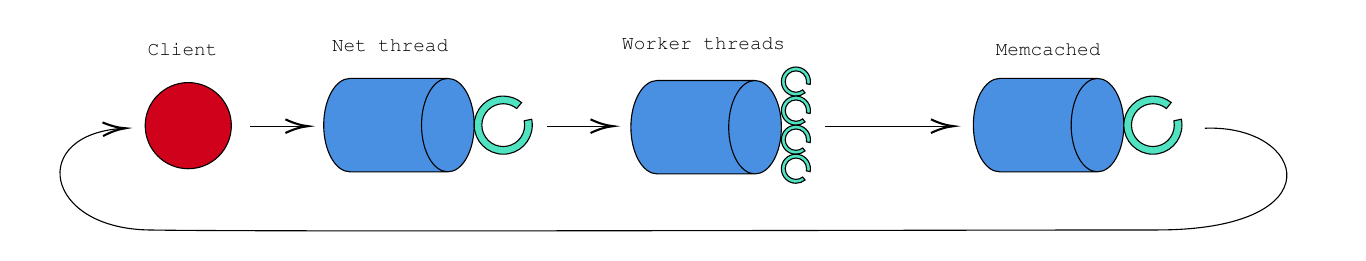
\begin{tikzpicture}[x=0.75pt,y=0.75pt,yscale=-1,xscale=1]
%uncomment if require: \path (0,300); %set diagram left start at 0, and has height of 300
%Shape: Circle [id:dp49354138354142396]
\draw  [fill={rgb, 255:red, 208; green, 2; blue, 27 }  ,fill opacity=1 ] (75,69.75) .. controls (75,58.29) and (84.29,49) .. (95.75,49) .. controls (107.21,49) and (116.5,58.29) .. (116.5,69.75) .. controls (116.5,81.21) and (107.21,90.5) .. (95.75,90.5) .. controls (84.29,90.5) and (75,81.21) .. (75,69.75) -- cycle ;
%Flowchart: Direct Access Storage [id:dp5740247909204759]
\draw  [fill={rgb, 255:red, 74; green, 144; blue, 226 }  ,fill opacity=1 ] (220.81,92) -- (173.69,92) .. controls (166.68,92) and (161,81.93) .. (161,69.5) .. controls (161,57.07) and (166.68,47) .. (173.69,47) -- (220.81,47)(233.5,69.5) .. controls (233.5,81.93) and (227.82,92) .. (220.81,92) .. controls (213.81,92) and (208.13,81.93) .. (208.13,69.5) .. controls (208.13,57.07) and (213.81,47) .. (220.81,47) .. controls (227.82,47) and (233.5,57.07) .. (233.5,69.5) ;
%Flowchart: Direct Access Storage [id:dp2829345888719481]
\draw  [fill={rgb, 255:red, 74; green, 144; blue, 226 }  ,fill opacity=1 ] (368.81,93) -- (321.69,93) .. controls (314.68,93) and (309,82.93) .. (309,70.5) .. controls (309,58.07) and (314.68,48) .. (321.69,48) -- (368.81,48)(381.5,70.5) .. controls (381.5,82.93) and (375.82,93) .. (368.81,93) .. controls (361.81,93) and (356.13,82.93) .. (356.13,70.5) .. controls (356.13,58.07) and (361.81,48) .. (368.81,48) .. controls (375.82,48) and (381.5,58.07) .. (381.5,70.5) ;
%Flowchart: Direct Access Storage [id:dp007966006600041098]
\draw  [fill={rgb, 255:red, 74; green, 144; blue, 226 }  ,fill opacity=1 ] (533.81,92) -- (486.69,92) .. controls (479.68,92) and (474,81.93) .. (474,69.5) .. controls (474,57.07) and (479.68,47) .. (486.69,47) -- (533.81,47)(546.5,69.5) .. controls (546.5,81.93) and (540.82,92) .. (533.81,92) .. controls (526.81,92) and (521.13,81.93) .. (521.13,69.5) .. controls (521.13,57.07) and (526.81,47) .. (533.81,47) .. controls (540.82,47) and (546.5,57.07) .. (546.5,69.5) ;
%Shape: Block Arc [id:dp5313515108315201]
\draw  [fill={rgb, 255:red, 80; green, 227; blue, 194 }  ,fill opacity=1 ] (261.21,66.66) .. controls (261.4,67.58) and (261.5,68.53) .. (261.5,69.5) .. controls (261.5,77.23) and (255.23,83.5) .. (247.5,83.5) .. controls (239.77,83.5) and (233.5,77.23) .. (233.5,69.5) .. controls (233.5,61.77) and (239.77,55.5) .. (247.5,55.5) .. controls (250.85,55.5) and (253.92,56.67) .. (256.33,58.63) -- (254,61.5) .. controls (252.23,60.06) and (249.96,59.19) .. (247.5,59.19) .. controls (241.81,59.19) and (237.19,63.81) .. (237.19,69.5) .. controls (237.19,75.19) and (241.81,79.81) .. (247.5,79.81) .. controls (253.19,79.81) and (257.81,75.19) .. (257.81,69.5) .. controls (257.81,68.78) and (257.73,68.09) .. (257.6,67.41) -- cycle ;
%Shape: Block Arc [id:dp8158443634034624]
\draw  [fill={rgb, 255:red, 80; green, 227; blue, 194 }  ,fill opacity=1 ] (395.36,49.92) .. controls (395.45,49.46) and (395.5,48.99) .. (395.5,48.5) .. controls (395.5,44.63) and (392.37,41.5) .. (388.5,41.5) .. controls (384.63,41.5) and (381.5,44.63) .. (381.5,48.5) .. controls (381.5,52.37) and (384.63,55.5) .. (388.5,55.5) .. controls (390.17,55.5) and (391.71,54.91) .. (392.91,53.93) -- (391.75,52.5) .. controls (390.86,53.22) and (389.73,53.65) .. (388.5,53.65) .. controls (385.65,53.65) and (383.35,51.35) .. (383.35,48.5) .. controls (383.35,45.65) and (385.65,43.35) .. (388.5,43.35) .. controls (391.35,43.35) and (393.65,45.65) .. (393.65,48.5) .. controls (393.65,48.86) and (393.62,49.21) .. (393.55,49.54) -- cycle ;
%Shape: Block Arc [id:dp17443429722166082]
\draw  [fill={rgb, 255:red, 80; green, 227; blue, 194 }  ,fill opacity=1 ] (395.36,63.92) .. controls (395.45,63.46) and (395.5,62.99) .. (395.5,62.5) .. controls (395.5,58.63) and (392.37,55.5) .. (388.5,55.5) .. controls (384.63,55.5) and (381.5,58.63) .. (381.5,62.5) .. controls (381.5,66.37) and (384.63,69.5) .. (388.5,69.5) .. controls (390.17,69.5) and (391.71,68.91) .. (392.91,67.93) -- (391.75,66.5) .. controls (390.86,67.22) and (389.73,67.65) .. (388.5,67.65) .. controls (385.65,67.65) and (383.35,65.35) .. (383.35,62.5) .. controls (383.35,59.65) and (385.65,57.35) .. (388.5,57.35) .. controls (391.35,57.35) and (393.65,59.65) .. (393.65,62.5) .. controls (393.65,62.86) and (393.62,63.21) .. (393.55,63.54) -- cycle ;
%Shape: Block Arc [id:dp2064055885735694]
\draw  [fill={rgb, 255:red, 80; green, 227; blue, 194 }  ,fill opacity=1 ] (395.36,77.92) .. controls (395.45,77.46) and (395.5,76.99) .. (395.5,76.5) .. controls (395.5,72.63) and (392.37,69.5) .. (388.5,69.5) .. controls (384.63,69.5) and (381.5,72.63) .. (381.5,76.5) .. controls (381.5,80.37) and (384.63,83.5) .. (388.5,83.5) .. controls (390.17,83.5) and (391.71,82.91) .. (392.91,81.93) -- (391.75,80.5) .. controls (390.86,81.22) and (389.73,81.65) .. (388.5,81.65) .. controls (385.65,81.65) and (383.35,79.35) .. (383.35,76.5) .. controls (383.35,73.65) and (385.65,71.35) .. (388.5,71.35) .. controls (391.35,71.35) and (393.65,73.65) .. (393.65,76.5) .. controls (393.65,76.86) and (393.62,77.21) .. (393.55,77.54) -- cycle ;
%Shape: Block Arc [id:dp4619516664271748]
\draw  [fill={rgb, 255:red, 80; green, 227; blue, 194 }  ,fill opacity=1 ] (395.36,91.92) .. controls (395.45,91.46) and (395.5,90.99) .. (395.5,90.5) .. controls (395.5,86.63) and (392.37,83.5) .. (388.5,83.5) .. controls (384.63,83.5) and (381.5,86.63) .. (381.5,90.5) .. controls (381.5,94.37) and (384.63,97.5) .. (388.5,97.5) .. controls (390.17,97.5) and (391.71,96.91) .. (392.91,95.93) -- (391.75,94.5) .. controls (390.86,95.22) and (389.73,95.65) .. (388.5,95.65) .. controls (385.65,95.65) and (383.35,93.35) .. (383.35,90.5) .. controls (383.35,87.65) and (385.65,85.35) .. (388.5,85.35) .. controls (391.35,85.35) and (393.65,87.65) .. (393.65,90.5) .. controls (393.65,90.86) and (393.62,91.21) .. (393.55,91.54) -- cycle ;
%Shape: Block Arc [id:dp1763104281611716]
\draw  [fill={rgb, 255:red, 80; green, 227; blue, 194 }  ,fill opacity=1 ] (574.21,66.66) .. controls (574.4,67.58) and (574.5,68.53) .. (574.5,69.5) .. controls (574.5,77.23) and (568.23,83.5) .. (560.5,83.5) .. controls (552.77,83.5) and (546.5,77.23) .. (546.5,69.5) .. controls (546.5,61.77) and (552.77,55.5) .. (560.5,55.5) .. controls (563.85,55.5) and (566.92,56.67) .. (569.33,58.63) -- (567,61.5) .. controls (565.23,60.06) and (562.96,59.19) .. (560.5,59.19) .. controls (554.81,59.19) and (550.19,63.81) .. (550.19,69.5) .. controls (550.19,75.19) and (554.81,79.81) .. (560.5,79.81) .. controls (566.19,79.81) and (570.81,75.19) .. (570.81,69.5) .. controls (570.81,68.78) and (570.73,68.09) .. (570.6,67.41) -- cycle ;
%Straight Lines [id:da6363213368613316]
\draw    (125.5,70) -- (151.5,70) ;
\draw [shift={(153.5,70)}, rotate = 180] [color={rgb, 255:red, 0; green, 0; blue, 0 }  ][line width=0.75]    (10.93,-3.29) .. controls (6.95,-1.4) and (3.31,-0.3) .. (0,0) .. controls (3.31,0.3) and (6.95,1.4) .. (10.93,3.29)   ;
%Straight Lines [id:da39568035783980227]
\draw    (268.5,70) -- (298.5,70) ;
\draw [shift={(300.5,70)}, rotate = 180] [color={rgb, 255:red, 0; green, 0; blue, 0 }  ][line width=0.75]    (10.93,-3.29) .. controls (6.95,-1.4) and (3.31,-0.3) .. (0,0) .. controls (3.31,0.3) and (6.95,1.4) .. (10.93,3.29)   ;
%Straight Lines [id:da9656074335554929]
\draw    (402.5,70) -- (462.5,70) ;
\draw [shift={(464.5,70)}, rotate = 180] [color={rgb, 255:red, 0; green, 0; blue, 0 }  ][line width=0.75]    (10.93,-3.29) .. controls (6.95,-1.4) and (3.31,-0.3) .. (0,0) .. controls (3.31,0.3) and (6.95,1.4) .. (10.93,3.29)   ;
%Curve Lines [id:da6184484614662842]
\draw    (585.5,71) .. controls (634.5,69) and (649.5,120) .. (562.5,120) .. controls (475.5,120) and (127.5,121) .. (76.5,120) .. controls (26.01,119.01) and (18.64,73.92) .. (64.11,71.07) ;
\draw [shift={(65.5,71)}, rotate = 537.56] [color={rgb, 255:red, 0; green, 0; blue, 0 }  ][line width=0.75]    (10.93,-3.29) .. controls (6.95,-1.4) and (3.31,-0.3) .. (0,0) .. controls (3.31,0.3) and (6.95,1.4) .. (10.93,3.29)   ;
% Text Node
\draw (193,31) node  [align=left] {{\scriptsize {\fontfamily{pcr}\selectfont Net thread}}};
% Text Node
\draw (344,30) node  [align=left] {{\fontfamily{pcr}\selectfont {\scriptsize Worker threads}}};
% Text Node
\draw (510,33) node  [align=left] {{\fontfamily{pcr}\selectfont {\scriptsize Memcached}}};
% Text Node
\draw (93,33) node  [align=left] {{\scriptsize {\fontfamily{pcr}\selectfont Client}}};
\end{tikzpicture}


Here is a table of the utilization that the algorithm gave us as output 
for both the read-only and write-only experiments, depending on the 
number of jobs that circulate in the system:

\begin{table}[H]
\centering
\begin{tabular}{@{}ccccccc@{}}
\toprule
\multicolumn{7}{c}{\textit{\textbf{Write-only workload}}} \\ \midrule
 & 6 jobs & 12 jobs & 24 jobs & 48 jobs & 96 jobs & 192 jobs \\ \midrule
\multicolumn{1}{c|}{Network thread} & 0.218 & 0.428 & 0.786 & 0.998 & 1.000 & 1.000 \\
\multicolumn{1}{c|}{Worker threads} & 0.004 & 0.008 & 0.015 & 0.019 & 0.019 & 0.019 \\
\multicolumn{1}{c|}{Server} & 0.169 & 0.330 & 0.607 & 0.771 & 0.772 & 0.772 \\ \midrule
\multicolumn{7}{c}{\textit{\textbf{Read-only workload}}} \\ \midrule
 & 6 jobs & 12 jobs & 24 jobs & 48 jobs & 96 jobs & 192 jobs \\ \midrule
\multicolumn{1}{c|}{Network thread} & 0.171 & 0.238 & 0.243 & 0.243 & 0.243 & 0.243 \\
\multicolumn{1}{c|}{Worker threads} & 0.003 & 0.004 & 0.005 & 0.005 & 0.005 & 0.005 \\
\multicolumn{1}{c|}{Server} & 0.705 & 0.982 & 1.000 & 1.000 & 1.000 & 1.000 \\ \bottomrule
\end{tabular}
\end{table}

We can immediately notice how in the read only experiment the bottleneck is the server, as
its utilization quickly gets very close to 1. This is in line with our findings in Section 2; in
fact, for the way we modeled the server, network latencies are included in the service time of
the server, so it makes sense that the server is highlighted as bottleneck.

For the write-only experiment, instead, we can see how the model highlights the bottleneck as 
the network thread, as its utilization gets very close to 1 from when there are 48 jobs in the system.

Worker threads have very low utilization values: this is because they do not comprehend network time, 
but only the cpu time needed to parse the request before sending it to the server. 



\subsubsection{Two middlewares}



\tikzset{every picture/.style={line width=0.75pt}} %set default line width to 0.75pt
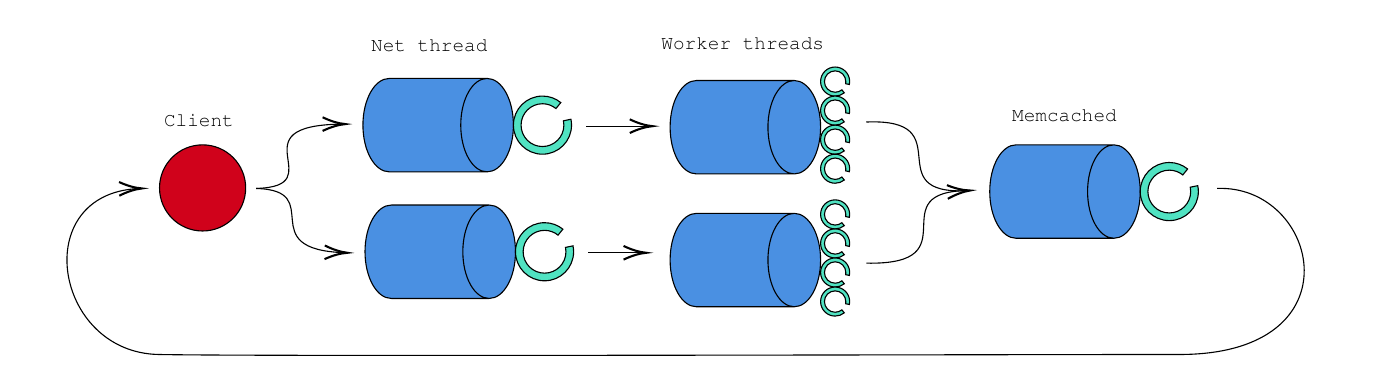
\begin{tikzpicture}[x=0.75pt,y=0.75pt,yscale=-1,xscale=1]
%uncomment if require: \path (0,300); %set diagram left start at 0, and has height of 300
%Shape: Circle [id:dp49354138354142396]
\draw  [fill={rgb, 255:red, 208; green, 2; blue, 27 }  ,fill opacity=1 ] (74,99.75) .. controls (74,88.29) and (83.29,79) .. (94.75,79) .. controls (106.21,79) and (115.5,88.29) .. (115.5,99.75) .. controls (115.5,111.21) and (106.21,120.5) .. (94.75,120.5) .. controls (83.29,120.5) and (74,111.21) .. (74,99.75) -- cycle ;
%Flowchart: Direct Access Storage [id:dp5740247909204759]
\draw  [fill={rgb, 255:red, 74; green, 144; blue, 226 }  ,fill opacity=1 ] (231.81,92) -- (184.69,92) .. controls (177.68,92) and (172,81.93) .. (172,69.5) .. controls (172,57.07) and (177.68,47) .. (184.69,47) -- (231.81,47)(244.5,69.5) .. controls (244.5,81.93) and (238.82,92) .. (231.81,92) .. controls (224.81,92) and (219.13,81.93) .. (219.13,69.5) .. controls (219.13,57.07) and (224.81,47) .. (231.81,47) .. controls (238.82,47) and (244.5,57.07) .. (244.5,69.5) ;
%Flowchart: Direct Access Storage [id:dp2829345888719481]
\draw  [fill={rgb, 255:red, 74; green, 144; blue, 226 }  ,fill opacity=1 ] (379.81,93) -- (332.69,93) .. controls (325.68,93) and (320,82.93) .. (320,70.5) .. controls (320,58.07) and (325.68,48) .. (332.69,48) -- (379.81,48)(392.5,70.5) .. controls (392.5,82.93) and (386.82,93) .. (379.81,93) .. controls (372.81,93) and (367.13,82.93) .. (367.13,70.5) .. controls (367.13,58.07) and (372.81,48) .. (379.81,48) .. controls (386.82,48) and (392.5,58.07) .. (392.5,70.5) ;
%Flowchart: Direct Access Storage [id:dp007966006600041098]
\draw  [fill={rgb, 255:red, 74; green, 144; blue, 226 }  ,fill opacity=1 ] (533.81,124) -- (486.69,124) .. controls (479.68,124) and (474,113.93) .. (474,101.5) .. controls (474,89.07) and (479.68,79) .. (486.69,79) -- (533.81,79)(546.5,101.5) .. controls (546.5,113.93) and (540.82,124) .. (533.81,124) .. controls (526.81,124) and (521.13,113.93) .. (521.13,101.5) .. controls (521.13,89.07) and (526.81,79) .. (533.81,79) .. controls (540.82,79) and (546.5,89.07) .. (546.5,101.5) ;
%Shape: Block Arc [id:dp5313515108315201]
\draw  [fill={rgb, 255:red, 80; green, 227; blue, 194 }  ,fill opacity=1 ] (272.21,66.66) .. controls (272.4,67.58) and (272.5,68.53) .. (272.5,69.5) .. controls (272.5,77.23) and (266.23,83.5) .. (258.5,83.5) .. controls (250.77,83.5) and (244.5,77.23) .. (244.5,69.5) .. controls (244.5,61.77) and (250.77,55.5) .. (258.5,55.5) .. controls (261.85,55.5) and (264.92,56.67) .. (267.33,58.63) -- (265,61.5) .. controls (263.23,60.06) and (260.96,59.19) .. (258.5,59.19) .. controls (252.81,59.19) and (248.19,63.81) .. (248.19,69.5) .. controls (248.19,75.19) and (252.81,79.81) .. (258.5,79.81) .. controls (264.19,79.81) and (268.81,75.19) .. (268.81,69.5) .. controls (268.81,68.78) and (268.73,68.09) .. (268.6,67.41) -- cycle ;
%Shape: Block Arc [id:dp8158443634034624]
\draw  [fill={rgb, 255:red, 80; green, 227; blue, 194 }  ,fill opacity=1 ] (406.36,49.92) .. controls (406.45,49.46) and (406.5,48.99) .. (406.5,48.5) .. controls (406.5,44.63) and (403.37,41.5) .. (399.5,41.5) .. controls (395.63,41.5) and (392.5,44.63) .. (392.5,48.5) .. controls (392.5,52.37) and (395.63,55.5) .. (399.5,55.5) .. controls (401.17,55.5) and (402.71,54.91) .. (403.91,53.93) -- (402.75,52.5) .. controls (401.86,53.22) and (400.73,53.65) .. (399.5,53.65) .. controls (396.65,53.65) and (394.35,51.35) .. (394.35,48.5) .. controls (394.35,45.65) and (396.65,43.35) .. (399.5,43.35) .. controls (402.35,43.35) and (404.65,45.65) .. (404.65,48.5) .. controls (404.65,48.86) and (404.62,49.21) .. (404.55,49.54) -- cycle ;
%Shape: Block Arc [id:dp17443429722166082]
\draw  [fill={rgb, 255:red, 80; green, 227; blue, 194 }  ,fill opacity=1 ] (406.36,63.92) .. controls (406.45,63.46) and (406.5,62.99) .. (406.5,62.5) .. controls (406.5,58.63) and (403.37,55.5) .. (399.5,55.5) .. controls (395.63,55.5) and (392.5,58.63) .. (392.5,62.5) .. controls (392.5,66.37) and (395.63,69.5) .. (399.5,69.5) .. controls (401.17,69.5) and (402.71,68.91) .. (403.91,67.93) -- (402.75,66.5) .. controls (401.86,67.22) and (400.73,67.65) .. (399.5,67.65) .. controls (396.65,67.65) and (394.35,65.35) .. (394.35,62.5) .. controls (394.35,59.65) and (396.65,57.35) .. (399.5,57.35) .. controls (402.35,57.35) and (404.65,59.65) .. (404.65,62.5) .. controls (404.65,62.86) and (404.62,63.21) .. (404.55,63.54) -- cycle ;
%Shape: Block Arc [id:dp2064055885735694]
\draw  [fill={rgb, 255:red, 80; green, 227; blue, 194 }  ,fill opacity=1 ] (406.36,77.92) .. controls (406.45,77.46) and (406.5,76.99) .. (406.5,76.5) .. controls (406.5,72.63) and (403.37,69.5) .. (399.5,69.5) .. controls (395.63,69.5) and (392.5,72.63) .. (392.5,76.5) .. controls (392.5,80.37) and (395.63,83.5) .. (399.5,83.5) .. controls (401.17,83.5) and (402.71,82.91) .. (403.91,81.93) -- (402.75,80.5) .. controls (401.86,81.22) and (400.73,81.65) .. (399.5,81.65) .. controls (396.65,81.65) and (394.35,79.35) .. (394.35,76.5) .. controls (394.35,73.65) and (396.65,71.35) .. (399.5,71.35) .. controls (402.35,71.35) and (404.65,73.65) .. (404.65,76.5) .. controls (404.65,76.86) and (404.62,77.21) .. (404.55,77.54) -- cycle ;
%Shape: Block Arc [id:dp4619516664271748]
\draw  [fill={rgb, 255:red, 80; green, 227; blue, 194 }  ,fill opacity=1 ] (406.36,91.92) .. controls (406.45,91.46) and (406.5,90.99) .. (406.5,90.5) .. controls (406.5,86.63) and (403.37,83.5) .. (399.5,83.5) .. controls (395.63,83.5) and (392.5,86.63) .. (392.5,90.5) .. controls (392.5,94.37) and (395.63,97.5) .. (399.5,97.5) .. controls (401.17,97.5) and (402.71,96.91) .. (403.91,95.93) -- (402.75,94.5) .. controls (401.86,95.22) and (400.73,95.65) .. (399.5,95.65) .. controls (396.65,95.65) and (394.35,93.35) .. (394.35,90.5) .. controls (394.35,87.65) and (396.65,85.35) .. (399.5,85.35) .. controls (402.35,85.35) and (404.65,87.65) .. (404.65,90.5) .. controls (404.65,90.86) and (404.62,91.21) .. (404.55,91.54) -- cycle ;
%Shape: Block Arc [id:dp1763104281611716]
\draw  [fill={rgb, 255:red, 80; green, 227; blue, 194 }  ,fill opacity=1 ] (574.21,98.66) .. controls (574.4,99.58) and (574.5,100.53) .. (574.5,101.5) .. controls (574.5,109.23) and (568.23,115.5) .. (560.5,115.5) .. controls (552.77,115.5) and (546.5,109.23) .. (546.5,101.5) .. controls (546.5,93.77) and (552.77,87.5) .. (560.5,87.5) .. controls (563.85,87.5) and (566.92,88.67) .. (569.33,90.63) -- (567,93.5) .. controls (565.23,92.06) and (562.96,91.19) .. (560.5,91.19) .. controls (554.81,91.19) and (550.19,95.81) .. (550.19,101.5) .. controls (550.19,107.19) and (554.81,111.81) .. (560.5,111.81) .. controls (566.19,111.81) and (570.81,107.19) .. (570.81,101.5) .. controls (570.81,100.78) and (570.73,100.09) .. (570.6,99.41) -- cycle ;
%Straight Lines [id:da39568035783980227]
\draw    (279.5,70) -- (309.5,70) ;
\draw [shift={(311.5,70)}, rotate = 180] [color={rgb, 255:red, 0; green, 0; blue, 0 }  ][line width=0.75]    (10.93,-3.29) .. controls (6.95,-1.4) and (3.31,-0.3) .. (0,0) .. controls (3.31,0.3) and (6.95,1.4) .. (10.93,3.29)   ;
%Curve Lines [id:da6184484614662842]
\draw    (583.5,100) .. controls (632.5,98) and (652.5,180) .. (565.5,180) .. controls (478.5,180) and (124.5,181) .. (73.5,180) .. controls (23.01,179.01) and (10.74,102.55) .. (63.87,100.05) ;
\draw [shift={(65.5,100)}, rotate = 538.96] [color={rgb, 255:red, 0; green, 0; blue, 0 }  ][line width=0.75]    (10.93,-3.29) .. controls (6.95,-1.4) and (3.31,-0.3) .. (0,0) .. controls (3.31,0.3) and (6.95,1.4) .. (10.93,3.29)   ;
%Flowchart: Direct Access Storage [id:dp7451835391522788]
\draw  [fill={rgb, 255:red, 74; green, 144; blue, 226 }  ,fill opacity=1 ] (379.81,157) -- (332.69,157) .. controls (325.68,157) and (320,146.93) .. (320,134.5) .. controls (320,122.07) and (325.68,112) .. (332.69,112) -- (379.81,112)(392.5,134.5) .. controls (392.5,146.93) and (386.82,157) .. (379.81,157) .. controls (372.81,157) and (367.13,146.93) .. (367.13,134.5) .. controls (367.13,122.07) and (372.81,112) .. (379.81,112) .. controls (386.82,112) and (392.5,122.07) .. (392.5,134.5) ;
%Shape: Block Arc [id:dp7380722475715134]
\draw  [fill={rgb, 255:red, 80; green, 227; blue, 194 }  ,fill opacity=1 ] (406.36,113.92) .. controls (406.45,113.46) and (406.5,112.99) .. (406.5,112.5) .. controls (406.5,108.63) and (403.37,105.5) .. (399.5,105.5) .. controls (395.63,105.5) and (392.5,108.63) .. (392.5,112.5) .. controls (392.5,116.37) and (395.63,119.5) .. (399.5,119.5) .. controls (401.17,119.5) and (402.71,118.91) .. (403.91,117.93) -- (402.75,116.5) .. controls (401.86,117.22) and (400.73,117.65) .. (399.5,117.65) .. controls (396.65,117.65) and (394.35,115.35) .. (394.35,112.5) .. controls (394.35,109.65) and (396.65,107.35) .. (399.5,107.35) .. controls (402.35,107.35) and (404.65,109.65) .. (404.65,112.5) .. controls (404.65,112.86) and (404.62,113.21) .. (404.55,113.54) -- cycle ;
%Shape: Block Arc [id:dp42502719835589375]
\draw  [fill={rgb, 255:red, 80; green, 227; blue, 194 }  ,fill opacity=1 ] (406.36,127.92) .. controls (406.45,127.46) and (406.5,126.99) .. (406.5,126.5) .. controls (406.5,122.63) and (403.37,119.5) .. (399.5,119.5) .. controls (395.63,119.5) and (392.5,122.63) .. (392.5,126.5) .. controls (392.5,130.37) and (395.63,133.5) .. (399.5,133.5) .. controls (401.17,133.5) and (402.71,132.91) .. (403.91,131.93) -- (402.75,130.5) .. controls (401.86,131.22) and (400.73,131.65) .. (399.5,131.65) .. controls (396.65,131.65) and (394.35,129.35) .. (394.35,126.5) .. controls (394.35,123.65) and (396.65,121.35) .. (399.5,121.35) .. controls (402.35,121.35) and (404.65,123.65) .. (404.65,126.5) .. controls (404.65,126.86) and (404.62,127.21) .. (404.55,127.54) -- cycle ;
%Shape: Block Arc [id:dp23264546060303126]
\draw  [fill={rgb, 255:red, 80; green, 227; blue, 194 }  ,fill opacity=1 ] (406.36,141.92) .. controls (406.45,141.46) and (406.5,140.99) .. (406.5,140.5) .. controls (406.5,136.63) and (403.37,133.5) .. (399.5,133.5) .. controls (395.63,133.5) and (392.5,136.63) .. (392.5,140.5) .. controls (392.5,144.37) and (395.63,147.5) .. (399.5,147.5) .. controls (401.17,147.5) and (402.71,146.91) .. (403.91,145.93) -- (402.75,144.5) .. controls (401.86,145.22) and (400.73,145.65) .. (399.5,145.65) .. controls (396.65,145.65) and (394.35,143.35) .. (394.35,140.5) .. controls (394.35,137.65) and (396.65,135.35) .. (399.5,135.35) .. controls (402.35,135.35) and (404.65,137.65) .. (404.65,140.5) .. controls (404.65,140.86) and (404.62,141.21) .. (404.55,141.54) -- cycle ;
%Shape: Block Arc [id:dp4280516951890485]
\draw  [fill={rgb, 255:red, 80; green, 227; blue, 194 }  ,fill opacity=1 ] (406.36,155.92) .. controls (406.45,155.46) and (406.5,154.99) .. (406.5,154.5) .. controls (406.5,150.63) and (403.37,147.5) .. (399.5,147.5) .. controls (395.63,147.5) and (392.5,150.63) .. (392.5,154.5) .. controls (392.5,158.37) and (395.63,161.5) .. (399.5,161.5) .. controls (401.17,161.5) and (402.71,160.91) .. (403.91,159.93) -- (402.75,158.5) .. controls (401.86,159.22) and (400.73,159.65) .. (399.5,159.65) .. controls (396.65,159.65) and (394.35,157.35) .. (394.35,154.5) .. controls (394.35,151.65) and (396.65,149.35) .. (399.5,149.35) .. controls (402.35,149.35) and (404.65,151.65) .. (404.65,154.5) .. controls (404.65,154.86) and (404.62,155.21) .. (404.55,155.54) -- cycle ;
%Curve Lines [id:da13510954714858103]
\draw    (414.5,136) .. controls (466.5,137) and (419.5,101) .. (464.5,101) ;
%Flowchart: Direct Access Storage [id:dp5070464595184729]
\draw  [fill={rgb, 255:red, 74; green, 144; blue, 226 }  ,fill opacity=1 ] (232.81,153) -- (185.69,153) .. controls (178.68,153) and (173,142.93) .. (173,130.5) .. controls (173,118.07) and (178.68,108) .. (185.69,108) -- (232.81,108)(245.5,130.5) .. controls (245.5,142.93) and (239.82,153) .. (232.81,153) .. controls (225.81,153) and (220.13,142.93) .. (220.13,130.5) .. controls (220.13,118.07) and (225.81,108) .. (232.81,108) .. controls (239.82,108) and (245.5,118.07) .. (245.5,130.5) ;
%Shape: Block Arc [id:dp6952384455522216]
\draw  [fill={rgb, 255:red, 80; green, 227; blue, 194 }  ,fill opacity=1 ] (273.21,127.66) .. controls (273.4,128.58) and (273.5,129.53) .. (273.5,130.5) .. controls (273.5,138.23) and (267.23,144.5) .. (259.5,144.5) .. controls (251.77,144.5) and (245.5,138.23) .. (245.5,130.5) .. controls (245.5,122.77) and (251.77,116.5) .. (259.5,116.5) .. controls (262.85,116.5) and (265.92,117.67) .. (268.33,119.63) -- (266,122.5) .. controls (264.23,121.06) and (261.96,120.19) .. (259.5,120.19) .. controls (253.81,120.19) and (249.19,124.81) .. (249.19,130.5) .. controls (249.19,136.19) and (253.81,140.81) .. (259.5,140.81) .. controls (265.19,140.81) and (269.81,136.19) .. (269.81,130.5) .. controls (269.81,129.78) and (269.73,129.09) .. (269.6,128.41) -- cycle ;
%Straight Lines [id:da4211032502689187]
\draw    (280.5,131) -- (306.5,131) ;
\draw [shift={(308.5,131)}, rotate = 180] [color={rgb, 255:red, 0; green, 0; blue, 0 }  ][line width=0.75]    (10.93,-3.29) .. controls (6.95,-1.4) and (3.31,-0.3) .. (0,0) .. controls (3.31,0.3) and (6.95,1.4) .. (10.93,3.29)   ;
%Curve Lines [id:da42521946433803426]
\draw    (120.5,100) .. controls (155.15,100.99) and (118.25,129.42) .. (163.12,130.96) ;
\draw [shift={(164.5,131)}, rotate = 181.22] [color={rgb, 255:red, 0; green, 0; blue, 0 }  ][line width=0.75]    (10.93,-3.29) .. controls (6.95,-1.4) and (3.31,-0.3) .. (0,0) .. controls (3.31,0.3) and (6.95,1.4) .. (10.93,3.29)   ;
%Curve Lines [id:da9569584611392035]
\draw    (120.5,100) .. controls (158.12,99.01) and (109.49,69.6) .. (161.88,69.01) ;
\draw [shift={(163.5,69)}, rotate = 180] [color={rgb, 255:red, 0; green, 0; blue, 0 }  ][line width=0.75]    (10.93,-3.29) .. controls (6.95,-1.4) and (3.31,-0.3) .. (0,0) .. controls (3.31,0.3) and (6.95,1.4) .. (10.93,3.29)   ;
%Curve Lines [id:da7738021817901635]
\draw    (414.5,68) .. controls (461.03,66.02) and (419.35,103.24) .. (463.15,101.08) ;
\draw [shift={(464.5,101)}, rotate = 536.27] [color={rgb, 255:red, 0; green, 0; blue, 0 }  ][line width=0.75]    (10.93,-3.29) .. controls (6.95,-1.4) and (3.31,-0.3) .. (0,0) .. controls (3.31,0.3) and (6.95,1.4) .. (10.93,3.29)   ;
% Text Node
\draw (204,31) node  [align=left] {{\scriptsize {\fontfamily{pcr}\selectfont Net thread}}};
% Text Node
\draw (355,30) node  [align=left] {{\fontfamily{pcr}\selectfont {\scriptsize Worker threads}}};
% Text Node
\draw (510,65) node  [align=left] {{\fontfamily{pcr}\selectfont {\scriptsize Memcached}}};
% Text Node
\draw (93,67) node  [align=left] {{\scriptsize {\fontfamily{pcr}\selectfont Client}}};
\end{tikzpicture}

(In red, delay centers; in blue, queues).

Here is a table of the utilization that the algorithm gave us as output 
for both the read-only and write-only experiments, depending on the 
number of jobs that circulate in the system:

\begin{table}[H]
\centering
\begin{tabular}{@{}ccccccc@{}}
\toprule
\multicolumn{7}{c}{\textit{\textbf{Write-only workload}}} \\ 
 & 6 jobs & 12 jobs & 24 jobs & 48 jobs & 96 jobs & 192 jobs \\ \midrule
\multicolumn{1}{c|}{Network thread} & 0.099 & 0.196 & 0.385 & 0.698 & 0.833 & 0.833 \\
\multicolumn{1}{c|}{Worker threads} & 0.001 & 0.003 & 0.006 & 0.010 & 0.012 & 0.012 \\
\multicolumn{1}{c|}{Server} & 0.119 & 0.236 & 0.462 & 0.838 & 1.000 & 1.000 \\ \midrule
\multicolumn{7}{c}{\textit{\textbf{Read-only workload}}} \\ 
 & 6 jobs & 12 jobs & 24 jobs & 48 jobs & 96 jobs & 192 jobs \\ \midrule
\multicolumn{1}{c|}{Network thread} & 0.085 & 0.142 & 0.156 & 0.156 & 0.156 & 0.156 \\
\multicolumn{1}{c|}{Worker threads} & 0.001 & 0.002 & 0.002 & 0.002 & 0.002 & 0.002 \\
\multicolumn{1}{c|}{Server} & 0.547 & 0.906 & 1.000 & 1.000 & 1.000 & 1.000 \\ \bottomrule
\end{tabular}
\end{table}

We have another confirmation of the server being the bottleneck in the read-only experiment.
But the more interesting part is the write-only experiment: we can see from the table very high
utilization values for both the network thread and the \t{memcached} server; however, ultimately
it is the server that gets flagged as the bottleneck. This is in line with our findings in the
summary of Section 4, when we found out that the majority of the response time of the middleware
is made of waiting for an answer from the server, not of the time spent in the job queue.


\subsubsection{Throughput estimates}

\begin{figure}[H]
	\begin{subfigure}[b]{0.5\linewidth}
		\includegraphics[width=\linewidth]{images/network/one_middleware.pdf}
	\end{subfigure}
	\begin{subfigure}[b]{0.5\linewidth}
		\includegraphics[width=\linewidth]{images/network/two_middlewares.pdf}
	\end{subfigure}
	\caption{On the left, predictions of the model for one middleware (write-only). 
	On the right, predictions of the model for two middlewares (write-only).}

	\label{fig:sharded}
\end{figure}

We can observe how both models are not very far off from the data measured from the experiments, 
but sometimes the trend are a bit different: in the one middleware configurations, the model 
gets completely saturated when there are 48 jobs, much more earlier than the real middleware.
The same thing happens with the two-middlewares model: the prediction gets saturated more quickly.

\end{document}
